\chapter{RESULTS AND DISCUSSIONS}
\label{chp:results-and-discussions}

In this chapter, methodology presented in this thesis study is applied on datasets and results are presented. Firstly, evaluation metrics are defined for each stage of methodology to evaluate performance of the approach. Following this, methodology is applied on two datasets and results are explained with discussions.

\section{Evaluation Metrics}
\label{sec:evaluation-metrics}
Approach in this study is an aggregation of various methods and they are significantly different from each other in their mathematical background. Therefore, instead of a global evaluation metric for the complete methodology, each stage will be evaluated within its evaluation metrics. Since these stages are executed sequentially, it is important for each stage to perform enough well to yield a successful outcome. In this section, evaluation metrics for each stage are presented and they will be used to determine the success of methodology on experiments.

\subsection{Process Model Mining}
\label{subsec:process-model-mining-eval}
Process model mining stage takes input as event logs of organizations and creates process models using process mining algorithms, which is \textit{Inductive Miner}\cite{leemans2014discoveringinfrequent} in this thesis. Performance of this stage can be measured by the conformance of the process models to the event logs. Four competing quality criteria are defined in \cite{van2011process} as \textit{fitness}, \textit{simplicity}, \textit{precision} and \textit{generalization}. Fitness is based on the idea of being able to replay event log over process model whereas precision focuses not underfitting the event log. Simplicity idea is based on the fact that the simplest model is the best model, on the other hand generalization supports not overfitting the event logs. These four competing criteria are mathematically defined in \cite{rozinat2008conformance} and grouped into two dimensions for analysis purposes:

\begin{description}
  \item[Fitness] Event log and the process model should \textit{fit} to each other, in other words process model should be able to parse the event log. 
  \item[Appropriateness] Since \textit{fitness} does not provide information about the meaningfulness of process models, this dimension is defined. Two notions comprise this idea; \textit{Structural Appropriateness} considers the simplicity whereas \textit{Behavioral Appropriateness} analyzes balance between overfitting and underfitting.
\end{description}

In this thesis study, process model mining stage will be evaluated by the \textit{Fitness} and \textit{Appropriateness} of the mined process models for each organization. It is expected to have higher \textit{fitness}, closer to 1, and a high level of appropriateness to continue to the next stages with the high quality process models. While evaluating, \textit{fitness} will be more dominant since \textit{appropriateness} without \textit{fitness} means less.
%	conformance plugin'i çağır, filtre ekranında var, 
%	structural olanı elle hesapla -> http://wwwis.win.tue.nl/~wvdaalst/publications/p436.pdf pg21
\subsection{Performance Indicator Analysis}
\label{subsec:performance-indicator-analysis-eval}
Performance indicator analysis stage consists of two parts as replaying event logs over process models and clustering organizations based on the performance indicators. In the replay phase, main operation is to \textit{align} \cite{van2012replaying} event logs and process models. This alignment is the based on the idea of finding the optimal alignment where total cost of \textit{move on process model} and \textit{move on event log} are minimized. Since there is no baseline information for alignment costs of organizational logs, total cost information will be used together with the process model mining evaluation metrics. In other words, for the event logs and process models with known conformance metrics, total cost of alignments will create a secondary check if there are any problems related to replaying events over process models. It is expected to have less total cost of alignment for the organizations with higher conformance since it is easy to align event logs and processes with higher fitness values.
% Şu pluginle bak: Check compliance using conformance checking ->

For the second stage of performance indicator analysis, there is a need to evaluate performance of clustering organizations. In this stage, organizations are clustered  based on their performance indicator values that are calculated over replaying. Since there is no labeled data in the context of this thesis study, any cross-validation techniques could not be applied and thus internal evaluation metrics are exploited. As mentioned in the Section~\ref{subsec:performance-indicator-clustering}, within-SSE values for clusters are plotted to the end user to select an appropriate number of clusters. It is expected that within-SSE values decreases as number of clusters increases; however, number of clusters should be selected without causing overfitting.
% wekadan gelen within sse 

\subsection{Mismatch Pattern Analysis}
\label{subsec:mismatch-pattern-analysis-eval}
Mismatch pattern analysis stage aims to find differences between the process models of different organizations. In this thesis study mismatch patterns defined in \cite{dijkman2007mismatch} are mathematically defined and analyzers are developed to locate these patterns. At the time of this study, it is known to be first to use mismatch patterns in a generic method, therefore evaluation is based on comparing with well-defined prior similarity metrics.

Structural similarity between process models is presented in \cite{dijkman2011similarity} by the \textit{graph-edit distance} notion. In graph theory, \textit{graph-edit distance} is the minimum number of \textit{graph-edit operations} necessary to get one graph from another. In process mining field, \textit{graph-edit operations} are simply node addition, deletion or substitution. In the study \cite{dijkman2011similarity}, both \textit{graph-edit distance} and \textit{graph-edit similarity} definitions are provided with their mathematical background. In this study, mismatch pattern analysis stage is evaluated by comparing the number of mismatch patterns and the \textit{graph-edit similarity} of process models. Without any performance indicator clustering, it is expected to have larger number of mismatch patterns when the similarity between process models is low. This will ensure the performance and suitability of using mismatch pattern analysis to spot differences of organizations' process models in the methodology.
 % BartHompes paketi ile ikili ikili çalıştır- run
\subsection{Recommendation Generation}
\label{subsec:recommendation-generation-eval}
In the recommendation generation stage, set of mismatch patterns are presented to end user based on the selected organization and performance difference threshold. This stage aims to list whole mismatch patterns that can cause the other organizations perform better than a difference threshold. Idea of using performance threshold should be evaluated in this stage with its responsiveness. In other words, it is expected that this stage will help the end user to focus on the most important performance improvements for the organization analyzed. Therefore, different threshold values will be tried to check how many mismatch patterns are generated for organizations and how they could be used for focused analysis. In addition, quality and applicability of the recommendations should be analyzed and this requires a high level of specialization. Knowledge required to analyze recommendations should include know-how about process changes, domain knowledge about the field of organizations' activity and structural attributions of the organizations.

\section{Dataset Selection}
\label{sec:dataset-selection}
Cross-organizational mining aims to find cross-correlation of workflows and activities in different organizations and this yields the necessity of organizations that do the same main activity with a comparable process flows. From the business environment point of view, this field needs alignment of the tasks from different organizations with different business needs, priorities and organizational structures and culture. Considering these characteristics, there are few dataset available in the literature that are well-structured, documented and valuable. In this thesis study, one synthetic and one real-life event log datasets are presented and used in the following sections to evaluate the performance of the proposed methodology.

\begin{description}
  \item[Loan Application Process \cite{loan-app-data}] This synthetically created dataset consists of event log variants of a simple loan application in a financial institute. In this application process, a customer fills a form and starts a request over website and it starts the different approaches of variants in different organizations that ends with notifying the customer about the acceptance of application. This dataset includes artificial event logs of 4 variants where each variant includes different sets of approaches such as parallelism, choices and sequential tasks. These event logs are used to test different approaches of discovering a configurable process model from a collection of event logs \cite{buijs2014flexible}.
  \item[Environmental Permit Application Process \cite{coselog-data}] This dataset originates from the "Configurable Services for Local Governments (CoSeLoG)" project \cite{van2011business} which investigates the similarities and dissimilarities between several processes of different municipalities in Netherlands.  Dataset contains records of the execution of receiving phase for the building permit application process in 5 municipalities, which are comparable since activity labels in the different event logs refer to the same activities performed in five municipalities. This dataset is also mentioned in the literature as \textit{"Processing applications for building and/or environmental permits (Wet Algemene Bepalingen omgevingsrecht (WABO) in Dutch)"}.

  When the organizations that have similar processes are considered, municipalities are one of the prominent candidates. In Netherlands there are more than 400 municipalities and they offer between 400 and 500 different products and services with their own processes. Unlike corporations, municipalities have the advantage that they can seek for collaboration since they are not direct competitions \cite{buijs2012towards} and this advantage makes them valuable for cross-organizational analysis. CoSeLoG research project aims to develop a business process management system within a shared Software-as-a-Service environment using the commonalities between the processes of municipalities \cite{buijs2014flexible}. In the scope of CoSeLoG research, five different processes of municipalities are analyzed and at the time of this thesis study only \textit{Environmental Permit Application Process} dataset is publicly shared.
\end{description}

\section{Loan Application Process}
\label{sec:loan-app-process}

\subsection{General Information}
\label{sec:loan-app-information}

In this section, methodology proposed in this thesis study will be applied on the \textit{Loan Application Process} dataset \cite{loan-app-data} and evaluation results will be presented. Statistical information about this dataset is presented in Table~\ref{table:loan-app-process-summary} to provide an insight about this dataset.
%\caption{Statistical summary of Loan Application Process Dataset}
%\label{table:loan-app-process-summary}
\begin{table}[]
\centering
\caption{Statistical summary of Loan Application Process dataset}
\label{table:loan-app-process-summary}
\begin{tabular}{@{}lccc@{}}
\toprule
                  & {\bf Cases} & {\bf Events} & {\bf Percentage} \\ \midrule
{\bf Variant \#1} & 100         & 590          & 24 \%            \\ \midrule
{\bf Variant \#2} & 70          & 420          & 17 \%            \\ \midrule
{\bf Variant \#3} & 200         & 800          & 33 \%            \\ \midrule
{\bf Variant \#4} & 105         & 630          & 26 \%            \\ \midrule
{\bf Total}       & {\bf 475}   & {\bf 2440}   & {\bf }           \\ \bottomrule
\end{tabular}
\end{table}

As shown in Table~\ref{table:loan-app-process-summary}, total of 475 cases and 2440 events included in this dataset with a fairly even distribution between variants. In the following section, these variants will be used as organizational logs and the methodology presented in this thesis study will be applied.

\subsection{Methodology Stages}
\label{sec:loan-app-methodology}
In \textit{Process Model Mining} stage, variants of the dataset are used as organizational event logs and they are used to mine process models. Since dataset is synthetically generated, noise threshold in \textit{Inductive Miner} is set to 0 and perfect log fitness is ensured. Appropriateness and fitness evaluation metrics are summarized in Table~\ref{table:loan-app-process-process-model-mining} and it can be seen that each event log is successful in terms of representing reality and being appropriate as a process model. Especially for the variants other than Variant \#1, there is a perfect fitness and appropriateness as it is expected from a  synthetically generated dataset without noise. In addition, process models for each event log is visualized in Figure~\ref{fig:loan-application-process-models}.
%\caption{Process Model Mining Evaluation of Loan Application Process Dataset}
%\label{table:loan-app-process-process-model-mining}
\begin{table}[]
\centering
\caption{Process Model Mining Evaluation of Loan Application Process Dataset}
\label{table:loan-app-process-process-model-mining}
\begin{tabular}{lcccc}
\hline
 & {\bf Fitness} & {\bf \begin{tabular}[c]{@{}c@{}}Structural\\Appropriateness\end{tabular}} & {\bf \begin{tabular}[c]{@{}c@{}}Behavioral\\Appropriateness\end{tabular}} & {\bf \begin{tabular}[c]{@{}c@{}}Average\\Appropriateness\end{tabular}} \\ \hline
{\bf Variant \#1} & 100 \% & 70 \% & 98.5 \% & 84.2 \% \\ \hline
{\bf Variant \#2} & 100 \% & 100 \% & 100 \% & 100 \% \\ \hline
{\bf Variant \#3} & 100 \% & 100 \% & 100 \% & 100 \% \\ \hline
{\bf Variant \#4} & 100 \% & 100 \% & 98.2 \% & 99.1 \% \\ \hline
{\bf Average} & {\bf 100 \%} & {\bf 92.5 \%} & {\bf 99.7 \%} & {\bf 96.06 \%} \\ \hline
\end{tabular}
\end{table}
\begin{figure}
\centering
  \begin{subfigure}{.4\textwidth}
    \centering
    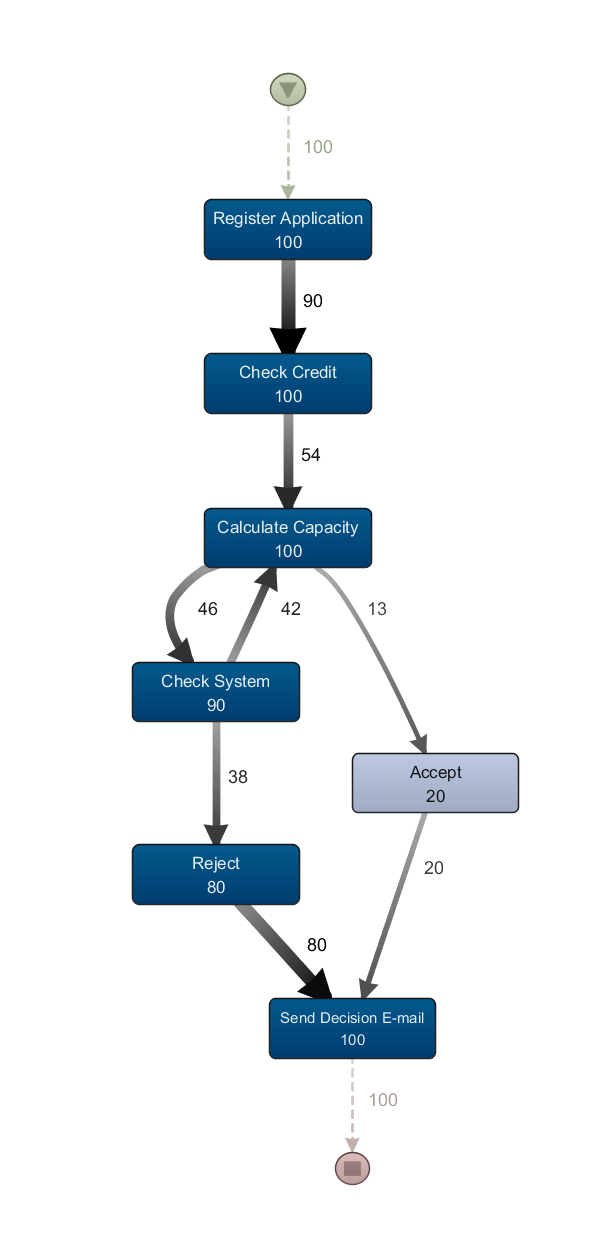
\includegraphics[width=.8\linewidth]{5_results_discussions/loan-application-process/ETM_Configuration1}
    \caption{Variant \#1}
    \label{fig:loan-application-process-models-1}
  \end{subfigure}%
  \begin{subfigure}{.4\textwidth}
    \centering
    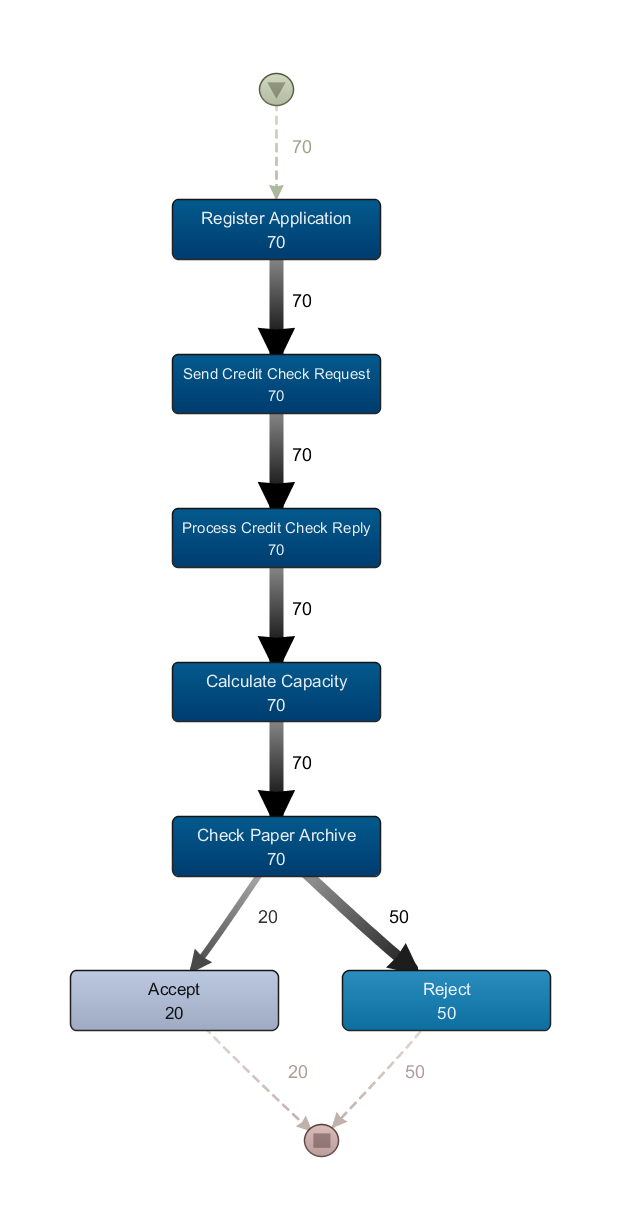
\includegraphics[width=.8\linewidth]{5_results_discussions/loan-application-process/ETM_Configuration2}
    \caption{Variant \#2}
    \label{fig:loan-application-process-models-2}
  \end{subfigure} \\
  \begin{subfigure}{.4\textwidth}
    \centering
    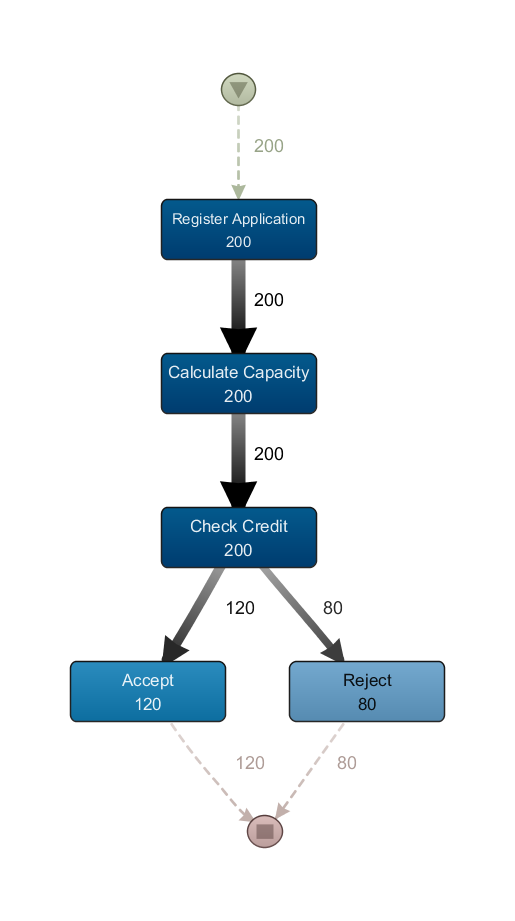
\includegraphics[width=.8\linewidth]{5_results_discussions/loan-application-process/ETM_Configuration3}
    \caption{Variant \#3}
    \label{fig:loan-application-process-models-3}
  \end{subfigure}%
  \begin{subfigure}{.4\textwidth}
    \centering
    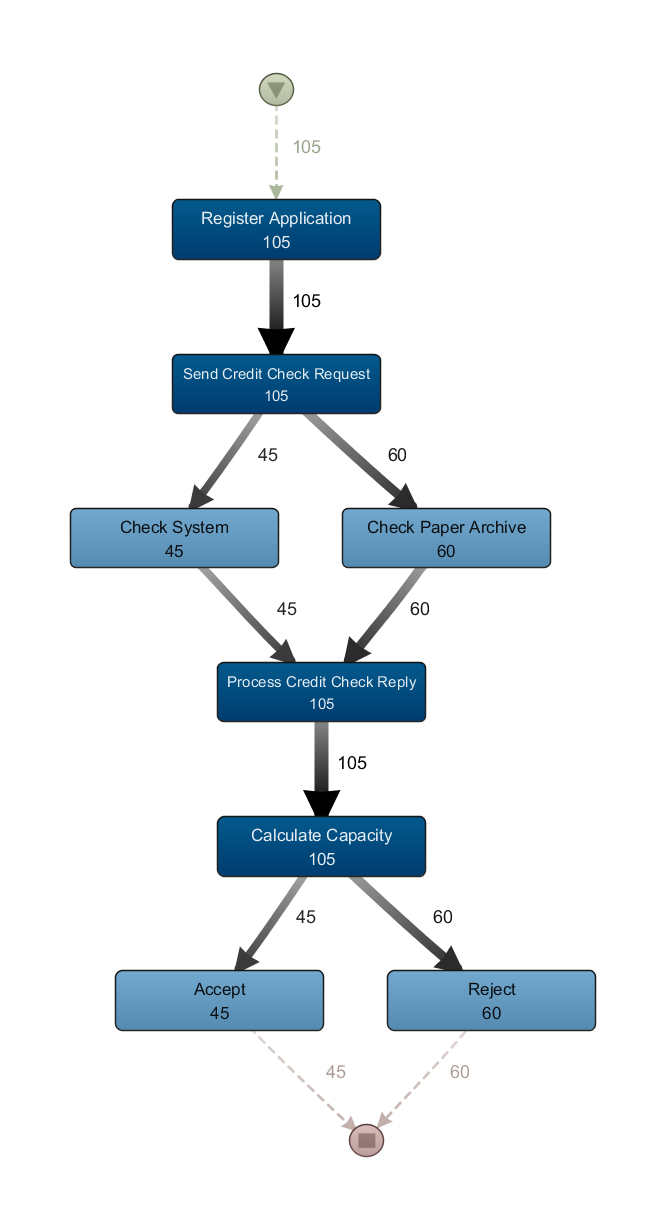
\includegraphics[width=.8\linewidth]{5_results_discussions/loan-application-process/ETM_Configuration4}
    \caption{Variant \#4}
    \label{fig:loan-application-process-models-4}
  \end{subfigure}
\caption{Process models of Loan Application Process dataset}
\label{fig:loan-application-process-models}
\end{figure} 

In \textit{Performance Indicator Analysis} stage, firstly event logs are replayed over process models and performance indicators are calculated. For replaying step, alignment costs should be checked with respect to process model mining evaluation metrics; however, since all fitness values of variants are 100 \% in Table~\ref{table:loan-app-process-process-model-mining}, corresponding alignment costs are 0 for this dataset. This ensures that event logs are successfully replayed over process models and performance indicators are calculated. With these performance indicators, organizations are clustered and internal evaluation of clusters are presented with different number of clusters in Figure~\ref{fig:loan-cluster-sse-plot}. As expected, within-SSE value decreases when number of clusters, \textit{k}, increases. Considering the effects of overfitting after the \textit{elbow} point in the plot, number of clusters is selected to be 2 for this dataset. For two clusters, Variant \#1, \#2, and \#4 are grouped into one cluster where only Variant \#3 is left to other cluster.
\begin{figure}
	\centering
	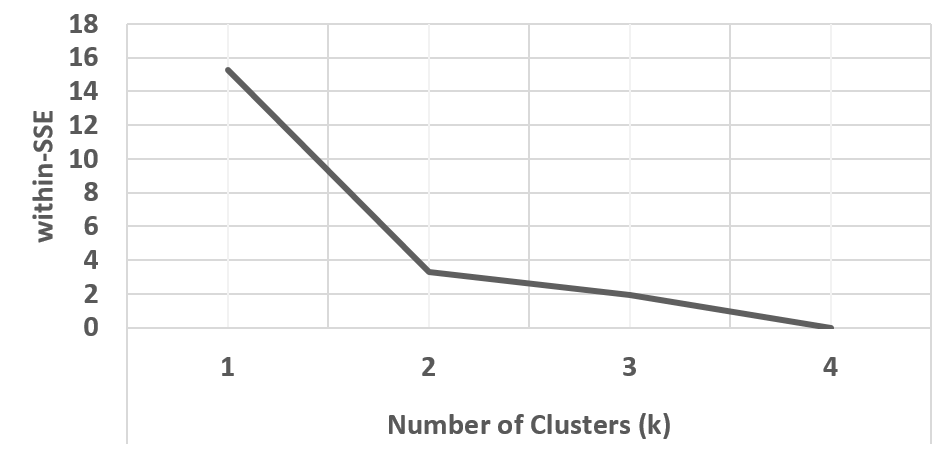
\includegraphics[width=.7\textwidth]{5_results_discussions/loan-application-process/cluster-sse-plot}
	\caption{Number of Clusters vs. within-SSE for Loan Application Process dataset}
  \label{fig:loan-cluster-sse-plot}
\end{figure}

In \textit{Mismatch Pattern Analysis} stage, number of mismatch patterns are analyzed with the \textit{graph-edit similarity} between each two organization. For each two organization, their \textit{graph-edit similarity} values are calculated and then our mismatch pattern analyzers are executed to spot differences. As the similarity between process models decreases our method spots more mismatch patterns for most of the variants and it ensures that the developed mismatch pattern analyzers work as expected for this dataset. Correlation between \textit{graph-edit similarity} and number of mismatch patterns are plotted in Figure~\ref{fig:loan-mismatch-pattern-analysis-results}.
\begin{figure}
	\centering
	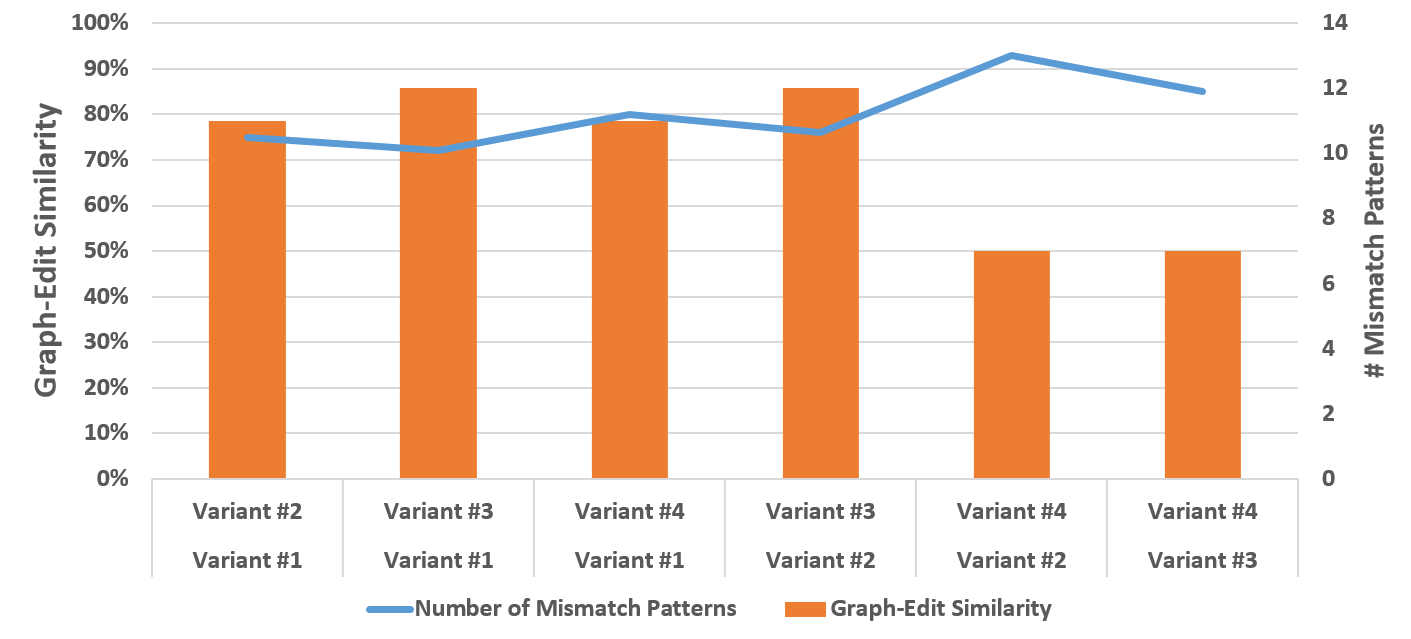
\includegraphics[width=\textwidth]{5_results_discussions/loan-application-process/mismatch-pattern-analysis-results}
	\caption{Mismatch Patterns vs. Graph-Edit Similarity for Loan Application Process variants}
  \label{fig:loan-mismatch-pattern-analysis-results}
\end{figure}

When the mismatch patterns are analyzed according to their types as diagrammed in Figure~\ref{fig:loan-mismatch-pattern-types}, \textit{"Skipped Activity"} and \textit{"Activities at Different Moments"} patterns are spotted mostly and no \textit{"Different Conditions for Occurrence"} or \textit{"Additional Dependencies"} patterns are discovered. Considering the small amount of this dataset, these numbers and distribution can be counted as acceptable in this stage of methodology.
\begin{figure}
	\centering
	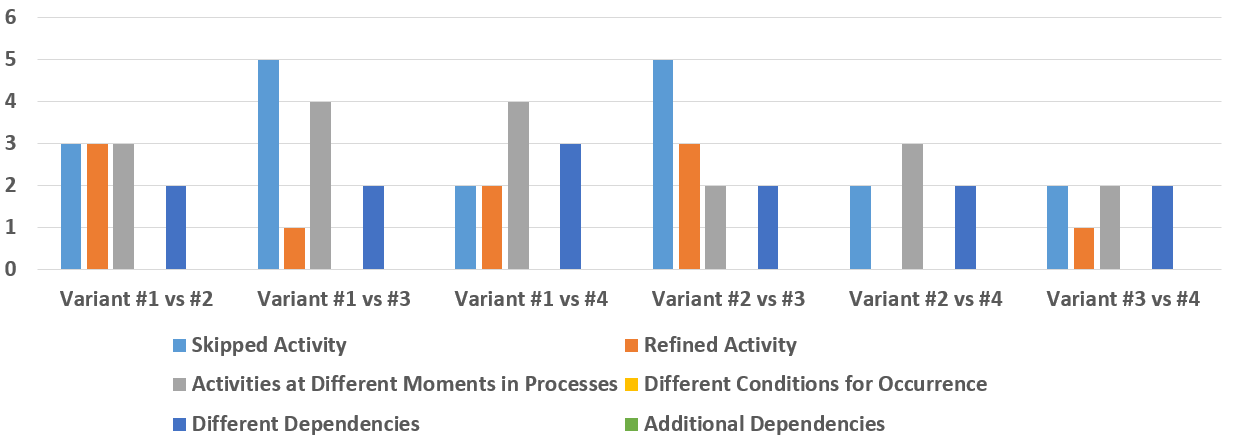
\includegraphics[width=\textwidth]{5_results_discussions/loan-application-process/mismatch-pattern-types}
	\caption{Mismatch pattern types for Loan Application Process variants}
  \label{fig:loan-mismatch-pattern-types}
\end{figure}
 
In \textit{Recommendation Generation} stage, an organization and performance difference threshold is selected as analysis input. For the selected organization's cluster, all other clusters are checked for performing better than the specified threshold. Instead of all mismatch patterns between organizations, only the mismatch patterns that are potential causes of other organizations to perform better are listed. For different threshold values, number of performance indicators that are performing better for the selected organization and spotted mismatch patterns are plotted in Figure~\ref{fig:loan-recommendation-generation-analysis}. 
\begin{figure}
	\centering
	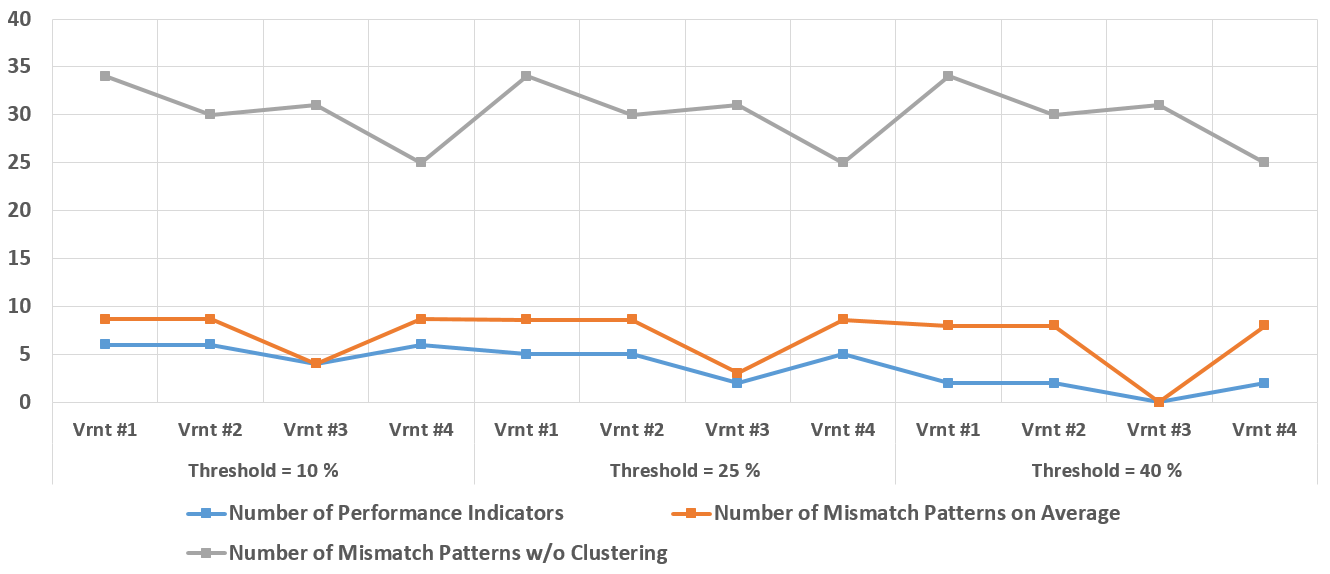
\includegraphics[width=\textwidth]{5_results_discussions/loan-application-process/recommendation-generation-analysis}
	\caption{Recommendation Generation analysis for Loan Application Process dataset}
  \label{fig:loan-recommendation-generation-analysis}
\end{figure}

In order to construct the data in Figure~\ref{fig:loan-recommendation-generation-analysis}, every organization is selected one-by-one with different threshold values. For every analysis, number of performance indicators and average number of mismatch patterns causing them are plotted. In addition, total number of mismatch patterns without clustering for each organization is added to the plot as an upper bound. With the help of this upper bound, responsiveness and degree of helping the user to focus on the performance improvement can be analyzed. As can be seen, for each threshold value, average number of mismatch patterns \textit{with performance indicator clustering} are very low compared to \textit{without clustering}. In other words, when user wants to improve its performance with any threshold, there is significantly less number of mismatch patterns on average to check. This shows the methodology proposed in this thesis can help users to focus on differences between organizations given this dataset. 
\section{Environmental Permit Application Process}
\label{sec:environmental-permit-application-process}
In this section, methodology proposed in this thesis study will be applied on the \textit{Environmental Permit Application Process} dataset \cite{coselog-data} and evaluation results will be presented with a similar approach above. Since this dataset consists of real-life event logs, preprocessing is undertaken prior to start analysis. Incomplete traces, which started but not ended in the time frame of log collection, and exceptional cases are removed from event logs with the help of ProM log visualization tools with a similar approach in \cite{buijs2014flexible}. Statistical information about the dataset that is used in this section can be summarized in Table~\ref{table:coselog-process-summary}.

%\caption{Statistical summary of Environmental Permit Application Process dataset}
%\label{table:coselog-process-summary}
 \begin{table}[]
\centering
\caption{Statistical summary of Environmental Permit Application Process dataset}
\label{table:coselog-process-summary}
\begin{tabular}{lccc}
\hline
                       & {\bf Cases} & {\bf Events} & {\bf Percentage} \\ \hline
{\bf Municipality \#1} & 54          & 131          & 6.1 \%           \\ \hline
{\bf Municipality \#2} & 302         & 586          & 27.3 \%          \\ \hline
{\bf Municipality \#3} & 37          & 73           & 3.4 \%           \\ \hline
{\bf Municipality \#4} & 340         & 507          & 23.7 \%          \\ \hline
{\bf Municipality \#5} & 481         & 845          & 39.4 \%          \\
{\bf Total}            & {\bf 1214}  & {\bf 2142}   & {\bf }           \\ \hline
\end{tabular}
\end{table}

As shown in Table~\ref{table:coselog-process-summary}, total of 1214 cases and 2142 events included in this dataset with a variable distribution between event logs of municipalities. In the following sections, these municipalities will be used as organizational logs and the methodology presented in this thesis study will be applied.

\subsection{Methodology Stages}
\label{sec:coselog-methodology}
In \textit{Process Model Mining} stage, event logs of each municipality in the dataset are used as organizational event logs and they are used to mine process models. Considering preprocessing is undertaken on the event logs, noise threshold in \textit{Inductive Miner} is set to a low value of 10\% to achieve a higher fitness. 

Appropriateness and fitness evaluation metrics are summarized in Table~\ref{table:coselog-wabo-process-model-mining} and it can be seen that each event log is successful in terms of representing reality with high fitness values. However, some of the process models like Municipality \#5 and \#4 resulted with low appropriateness values. Process models for each event log are visualized with a detail simplification based on number of activities and paths in Figure~\ref{fig:coselog-wabo-process-models} and it can be seen that low appropriateness values resulted with complicated process models that are difficult to analyze visually. Detail simplification is only used for visualization and it draws the mainstream process flows instead of whole set of paths and activities. It should be kept in mind that actual process models are 10 to 20 times more complicated in terms of number of activities and paths than the ones presented in Figure~\ref{fig:coselog-wabo-process-models}. 
%\caption{Process Model Mining Evaluation of Environmental Permit Application Process Dataset}
%\label{table:coselog-wabo-process-model-mining}
\begin{table}[]
\centering
\caption{Process Model Mining Evaluation of Environmental Permit Application Process Dataset}
\label{table:coselog-wabo-process-model-mining}
\begin{tabular}{lcccc}
\hline
 & {\bf Fitness} & {\bf \begin{tabular}[c]{@{}c@{}}Structural\\Appropriateness\end{tabular}} & {\bf \begin{tabular}[c]{@{}c@{}}Behavioral\\Appropriateness\end{tabular}} & {\bf \begin{tabular}[c]{@{}c@{}}Average\\Appropriateness\end{tabular}} \\ \hline
{\bf Municipality \#1} & 86 \% & 97.5 \% & 54.4 \% & 76 \% \\ \hline
{\bf Municipality \#2} & 100 \% & 100 \% & 100 \% & 100 \% \\ \hline
{\bf Municipality \#3} & 92.3 \% & 71.1 \% & 67.2 \% & 69.1 \% \\ \hline
{\bf Municipality \#4} & 96.8 \% & 65.7 \% & 64 \% & 64.9 \% \\ \hline
{\bf Municipality \#5} & 94.5 \% & 58.8 \% & 39.7 \% & 49.3 \% \\ \hline
{\bf Average} & {\bf 93.9 \%} & {\bf 78.6 \%} & {\bf 65.1 \%} & {\bf 71.9 \%} \\ \hline
\end{tabular}
\end{table}

\begin{figure}[]
\centering
  \begin{subfigure}{.4\textwidth}
    \centering
    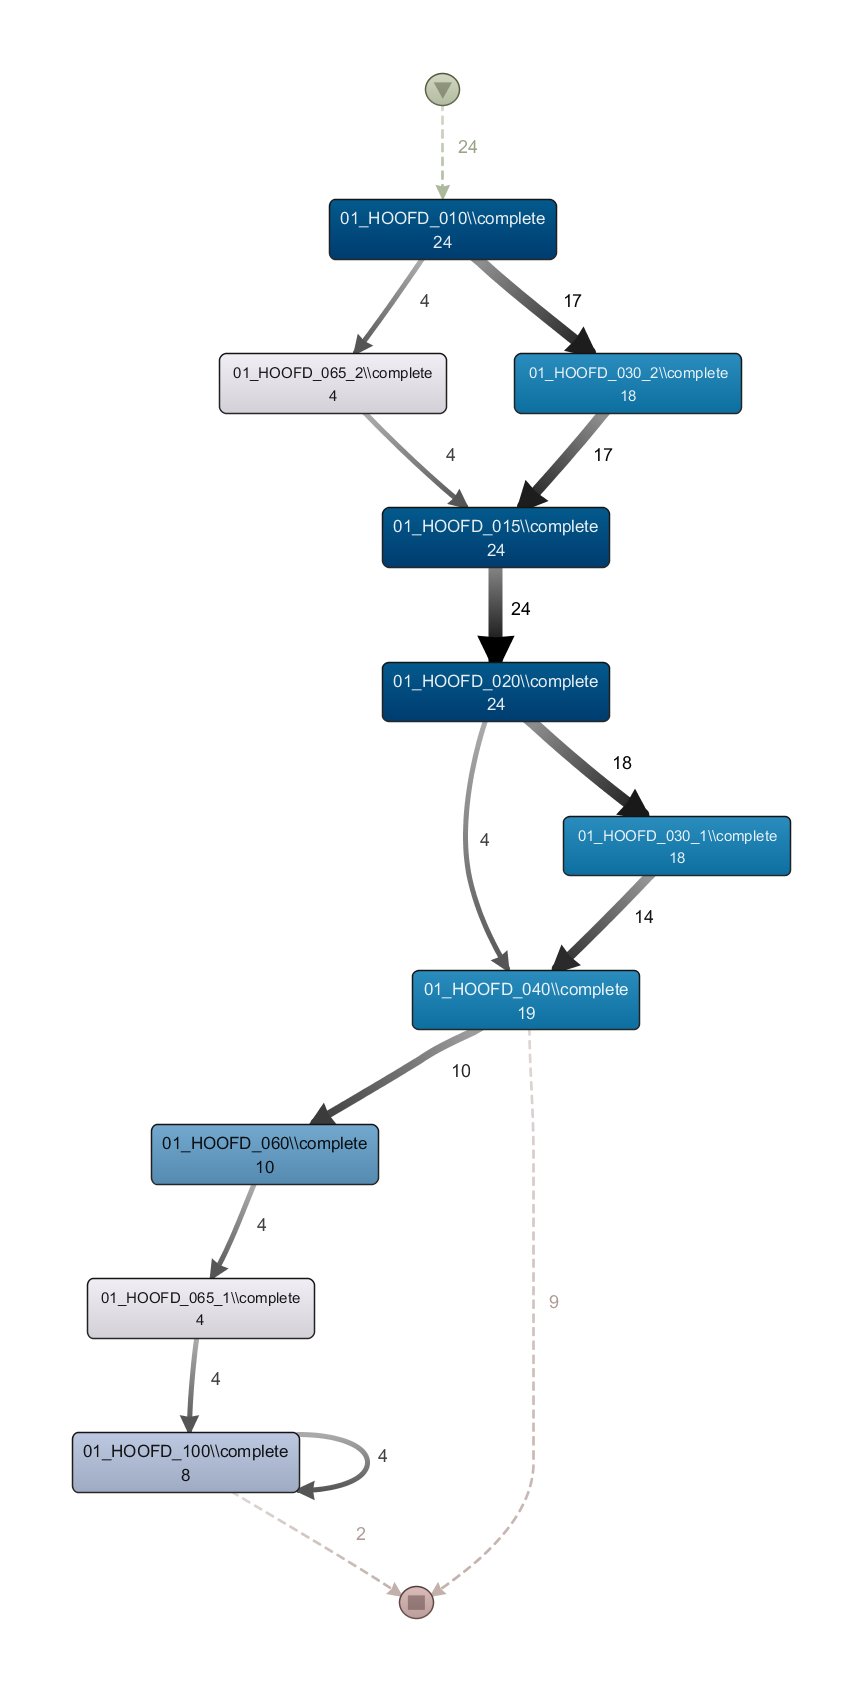
\includegraphics[width=.8\linewidth]{5_results_discussions/coselog-wabo/coselog-wabo-1-simplified}
    \caption{Municipality \#1}
    \label{fig:coselog-wabo-process-models-simplified-1}
  \end{subfigure}%
  \begin{subfigure}{.2\textwidth}
    \centering
    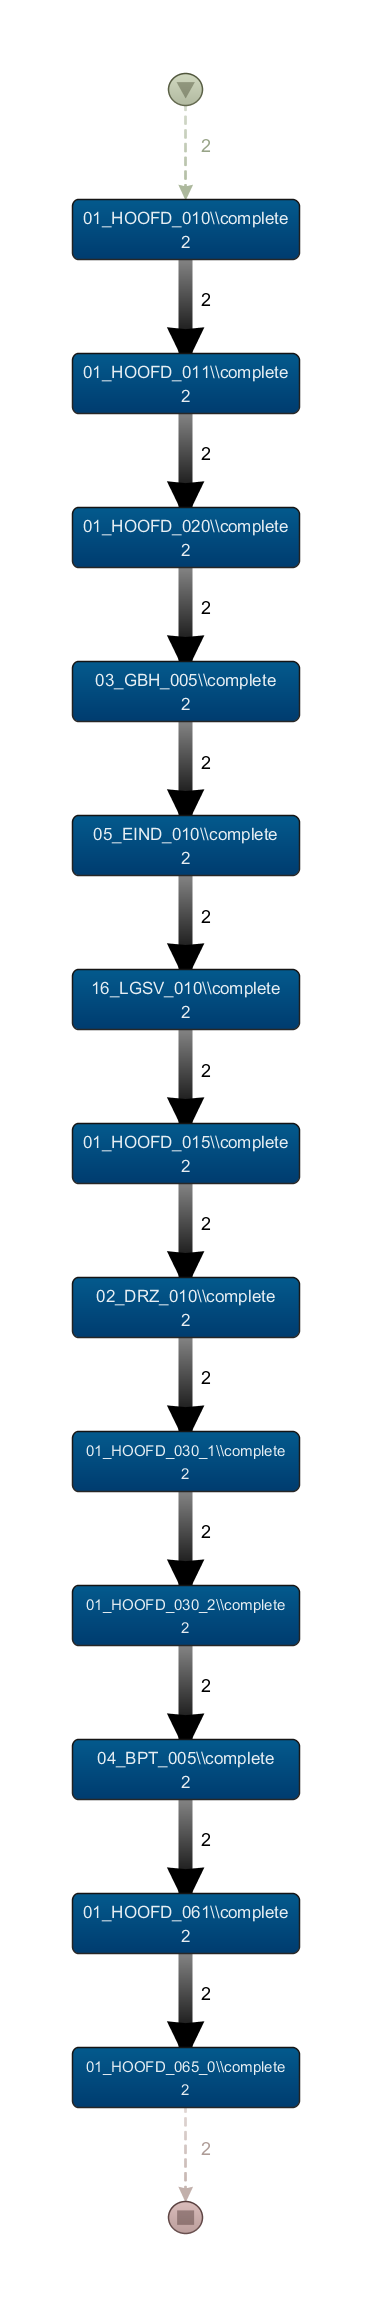
\includegraphics[width=.5\linewidth]{5_results_discussions/coselog-wabo/coselog-wabo-2-simplified}
    \caption{Municipality \#2}
    \label{fig:coselog-wabo-process-models-simplified-2}
  \end{subfigure} 
  \begin{subfigure}{.3\textwidth}
    \centering
        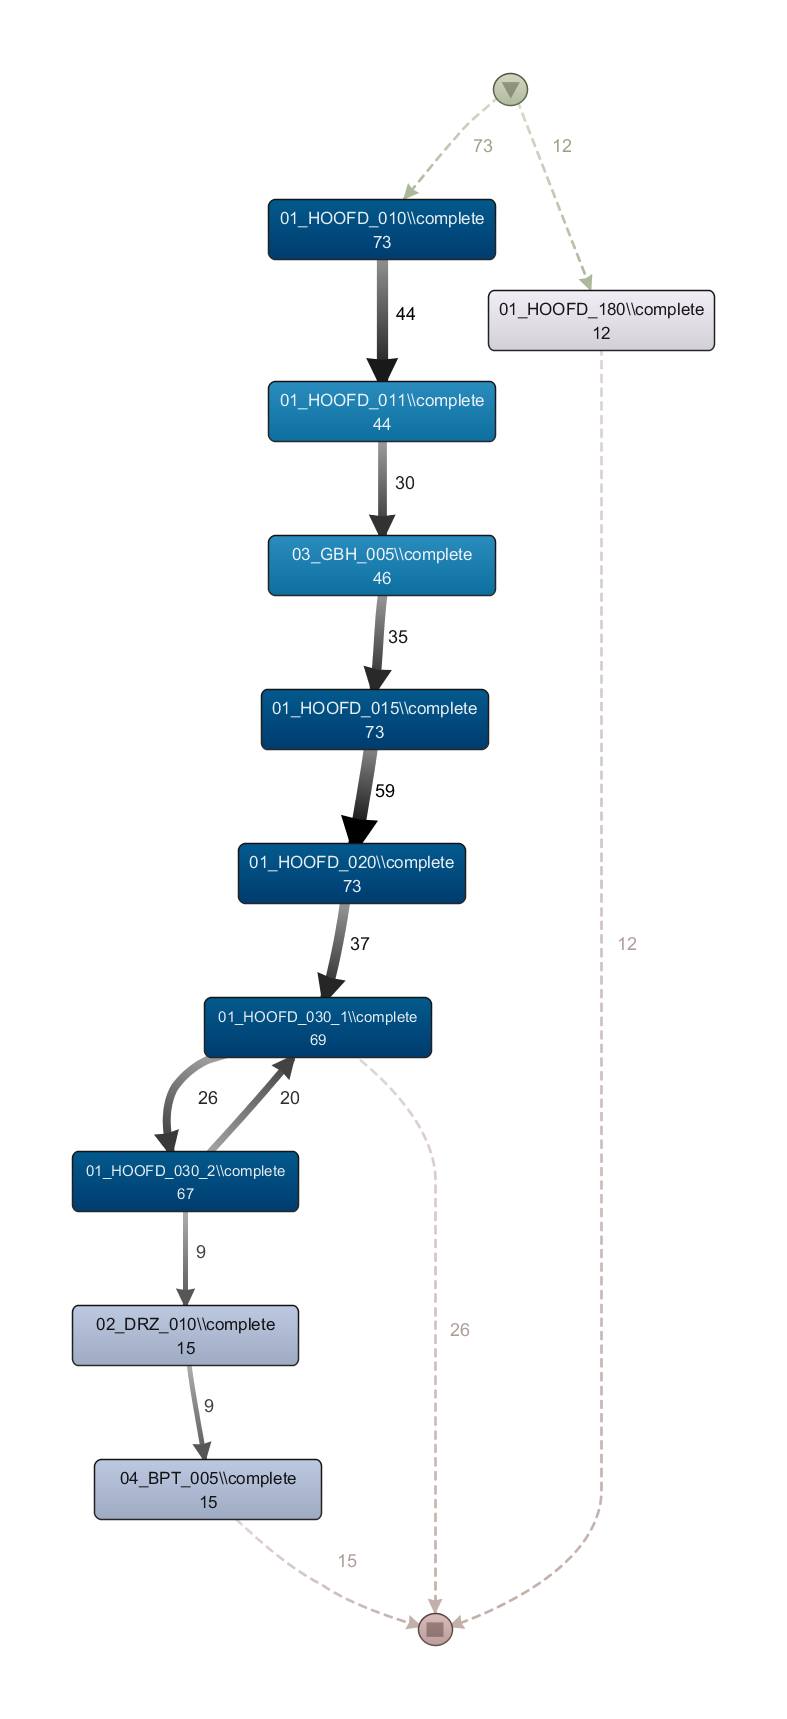
\includegraphics[width=.8\linewidth]{5_results_discussions/coselog-wabo/coselog-wabo-3-simplified}
    \caption{Municipality \#3}
    \label{fig:coselog-wabo-process-models-simplified-3}
  \end{subfigure} 
  \begin{subfigure}{.4\textwidth}
    \centering
        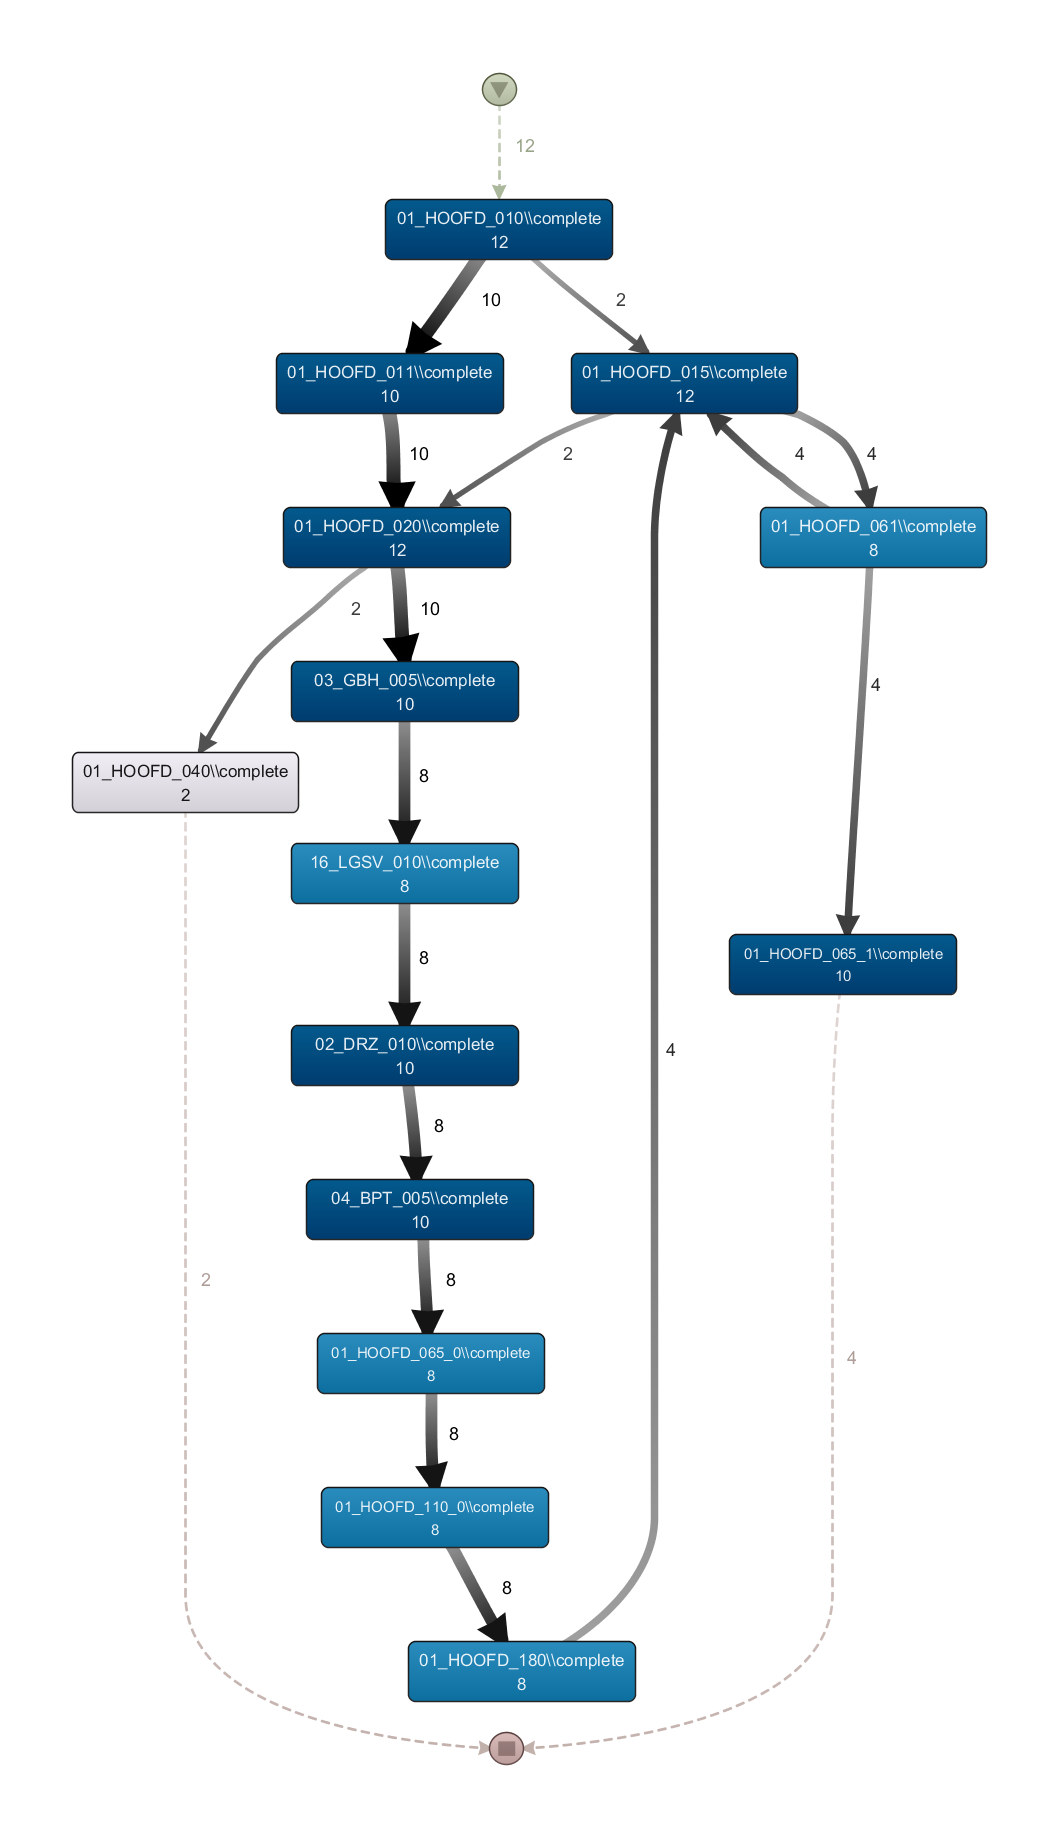
\includegraphics[width=.8\linewidth]{5_results_discussions/coselog-wabo/coselog-wabo-4-simplified}
    \caption{Municipality \#5}
    \label{fig:coselog-wabo-process-models-simplified-4}
  \end{subfigure}
    \begin{subfigure}{.4\textwidth}
    \centering
        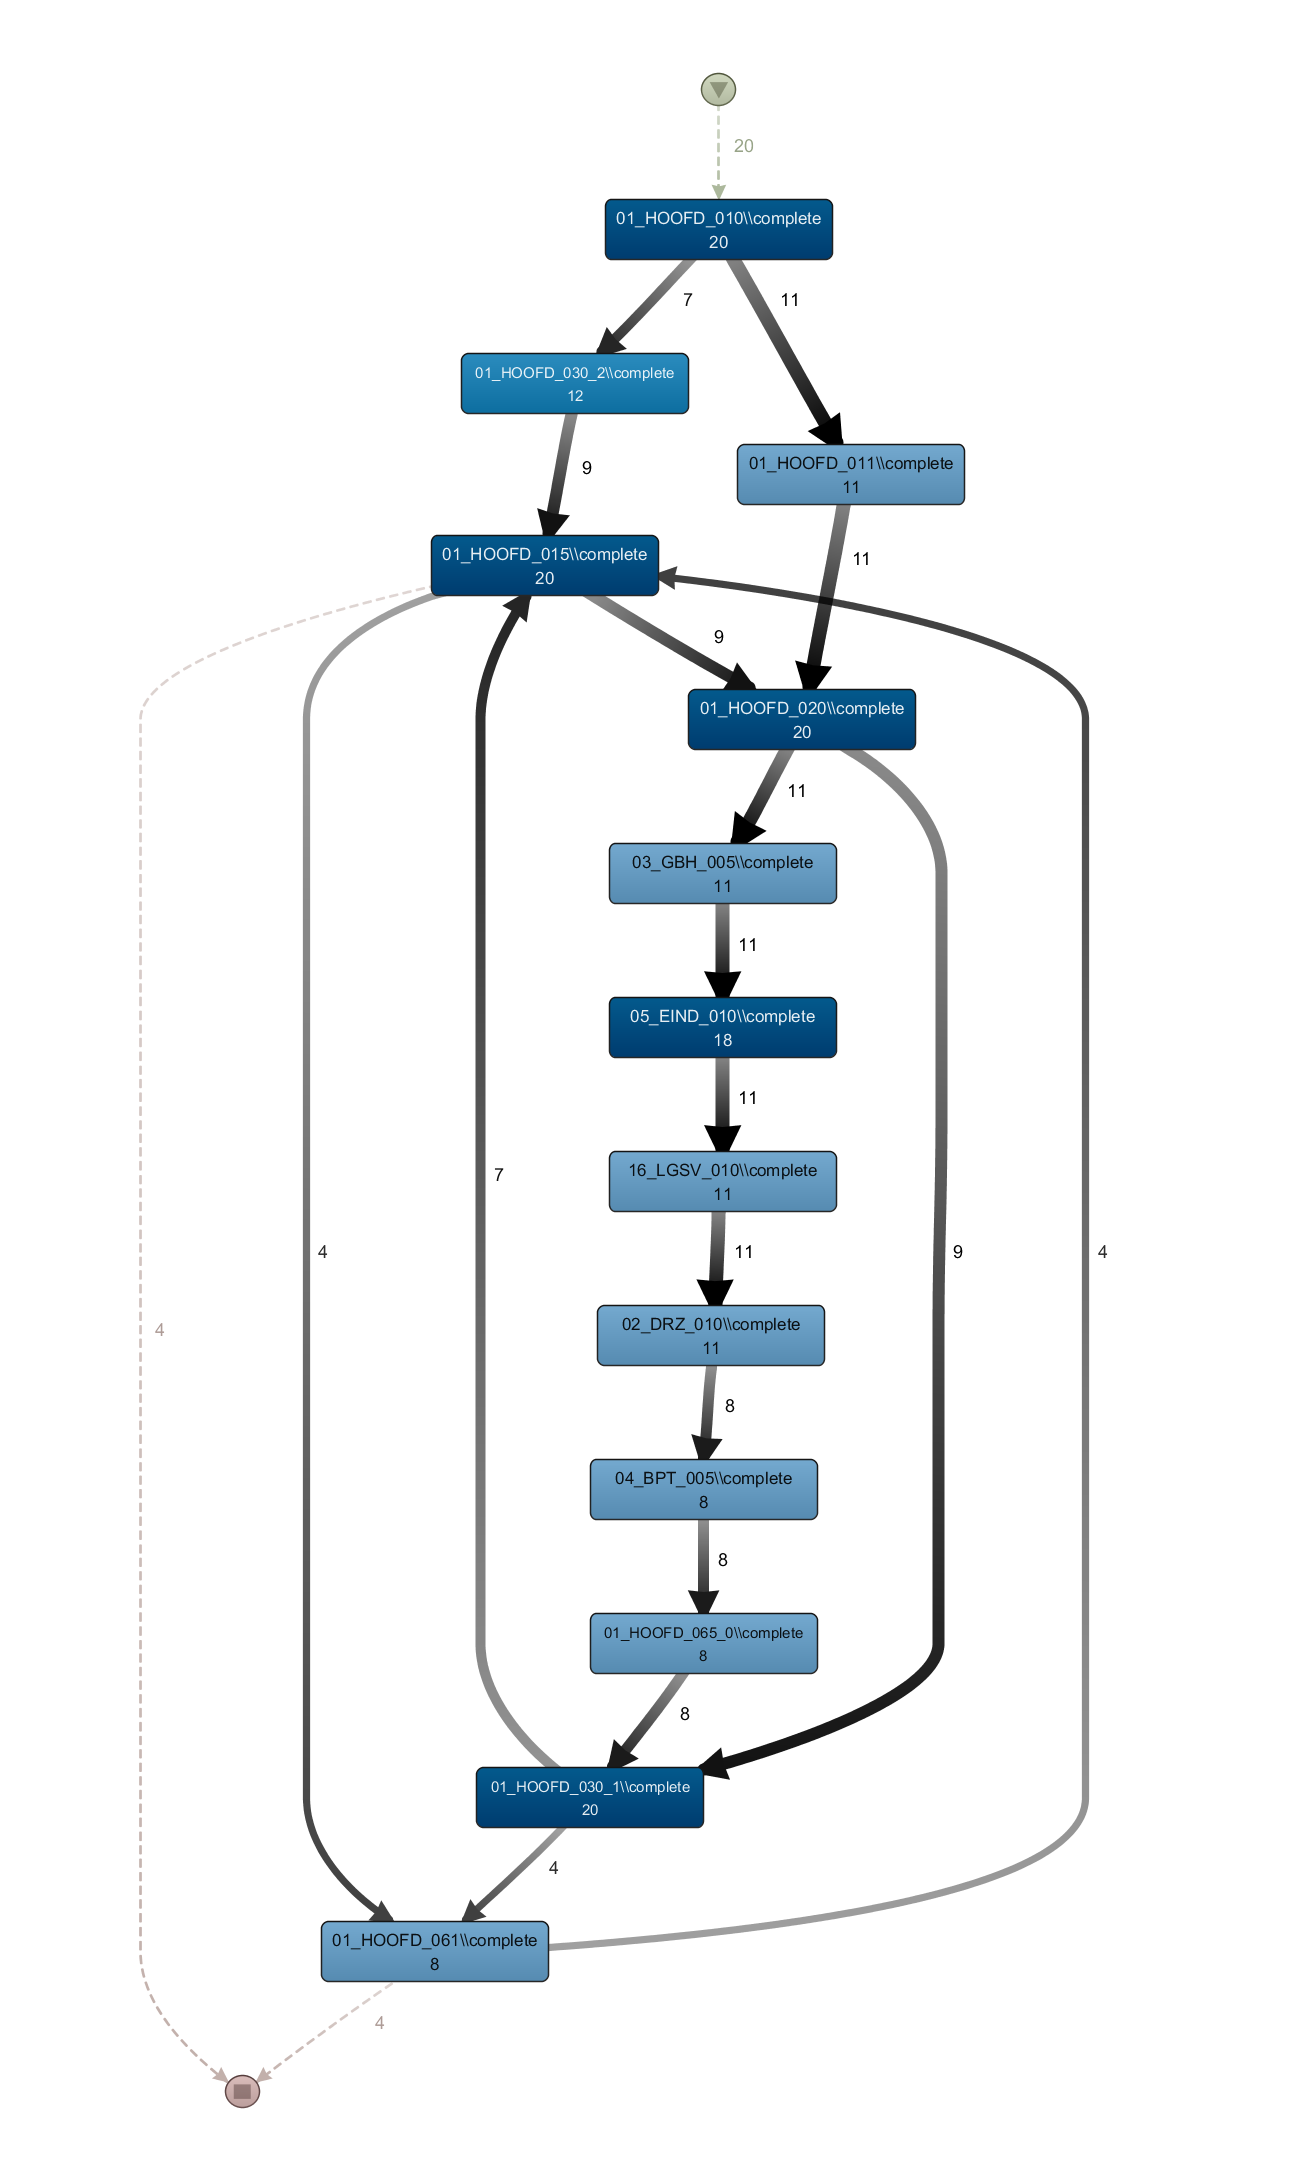
\includegraphics[width=.8\linewidth]{5_results_discussions/coselog-wabo/coselog-wabo-5-simplified}
    \caption{Municipality \#5}
    \label{fig:coselog-wabo-process-models-simplified-5}
  \end{subfigure}%
\caption{Process models of Environmental Permit Application Process Dataset}
\label{fig:coselog-wabo-process-models}
\end{figure} 



In \textit{Performance Indicator Analysis} stage, alignment costs are calculated over replay of event logs on process models. As presented in the Table~\ref{table:coselog-wabo-replay}, as appropriateness and fitness decrease alignment costs increase for the municipalities. This indicates the fact that both process model mining stage and replay stage is in conformity and performance indicators calculated over replay are acceptable.
%\caption{Replay Evaluation of Environmental Permit Application Process Dataset}
%\label{table:coselog-wabo-replay}
\begin{table}[]
\centering
\caption{Replay Evaluation of Environmental Permit Application Process Dataset}
\label{table:coselog-wabo-replay}
\begin{tabular}{lccc}
\hline
 & {\bf Fitness} & {\bf Average Appropriateness} & {\bf Alignment Cost} \\ \hline
{\bf Municipality \#1} & 86 \% & 76 \% & 173.2 \\ \hline
{\bf Municipality \#2} & 100 \% & 100 \% & 0 \\ \hline
{\bf Municipality \#3} & 92,3 \% & 69,1 \% & 332.3 \\ \hline
{\bf Municipality \#4} & 96,8 \% & 64,9 \% & 9,1 \\ \hline
{\bf Municipality \#5} & 94,5 \% & 49,3 \% & 35.8 \\ \hline
\end{tabular}
\end{table}

After calculating the performance indicators, municipalities are clustered based on these values and this stage is evaluated by the within-SSE values for different number of clusters as plotted in Figure~\ref{fig:coselog-wabo-cluster-sse-plot}. In order to avoid overfitting of clusters, number of clusters, \textit{k}, is selected to be 2 for this dataset for further analysis. For two clusters, Municipality \#1 is located in one cluster where municipalities \#2, \#3, \#4 and \#5 are grouped into to other cluster.
\begin{figure}
	\centering
	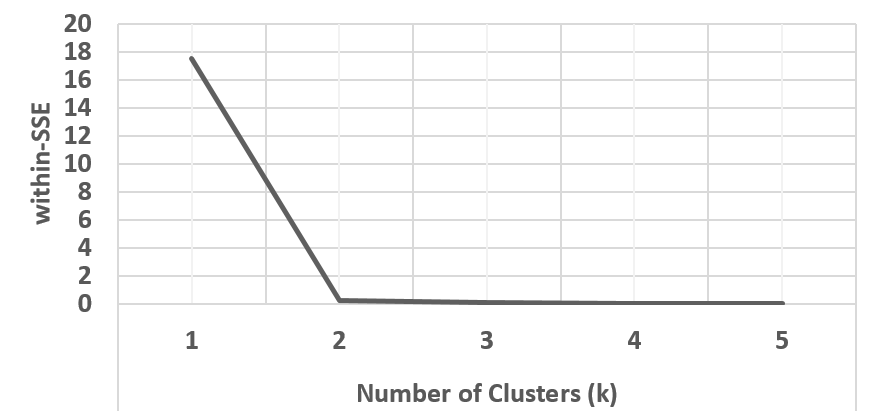
\includegraphics[width=.7\textwidth]{5_results_discussions/coselog-wabo/cluster-sse-plot}
	\caption{Number of Clusters vs. within-SSE for Environmental Permit Application Process Dataset}
  \label{fig:coselog-wabo-cluster-sse-plot}
\end{figure}

In \textit{Mismatch Pattern Analysis} stage, number of mismatch patterns are analyzed with the \textit{graph-edit similarity} between each two municipality. In order to check correlation between \textit{graph-edit similarity} and number of mismatch patterns, data is plotted in Figure~\ref{fig:coselog-wabo-pattern-analysis-results}. When the plot is checked, it can be seen that as the similarity between process models of municipalities increases, number of mismatch patterns decreases on most of the cases. When further analyzed, it can be seen that Municipalities \#4 and \#5, which have significantly more complex process model compared to others, fails in spotting mismatch patterns according to \textit{graph-edit similarity}.
\begin{figure}
	\centering
	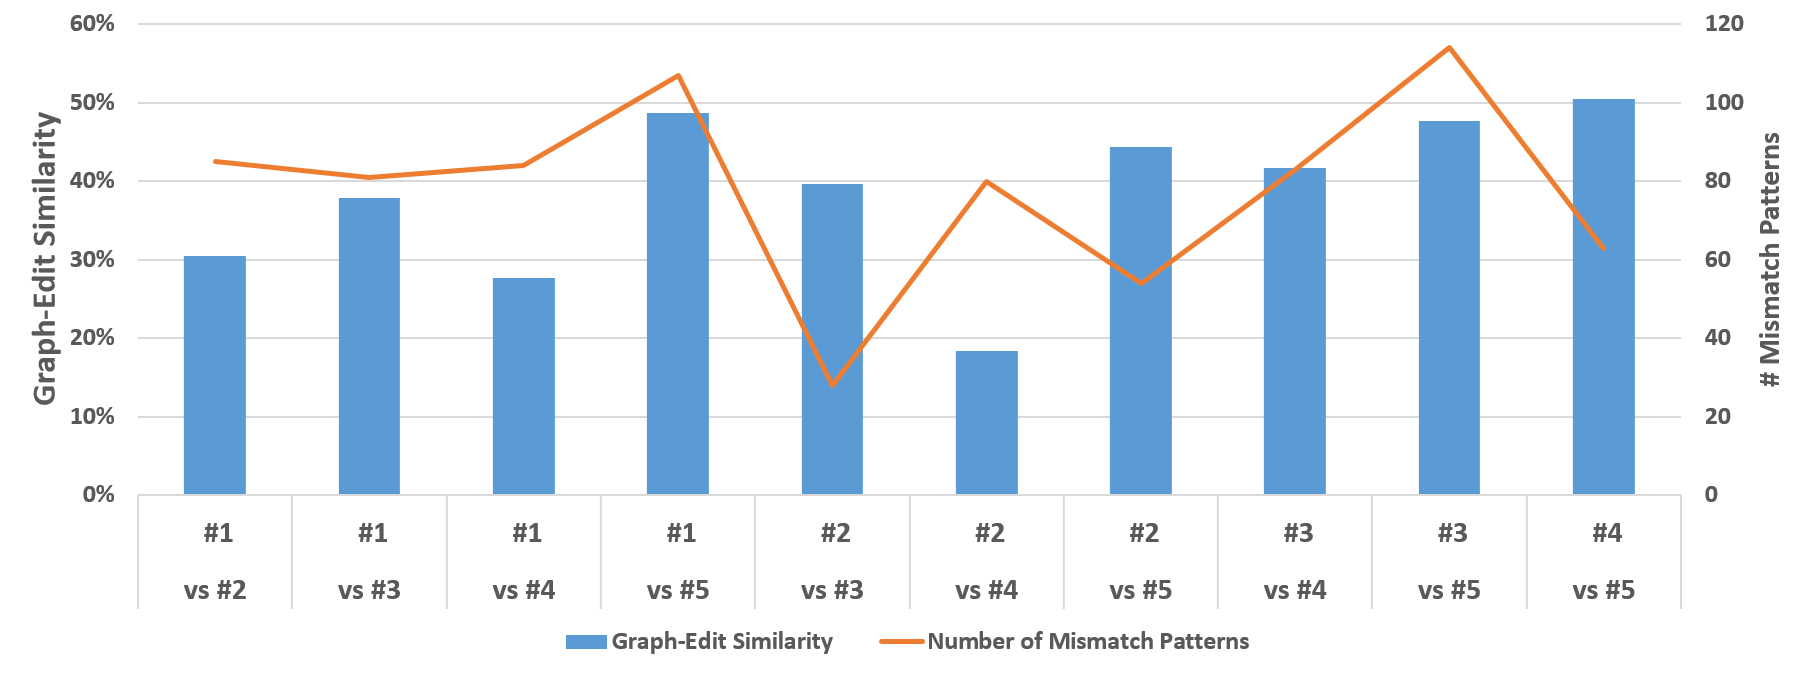
\includegraphics[width=\textwidth]{5_results_discussions/coselog-wabo/mismatch-pattern-analysis-results}
	\caption{Mismatch Patterns vs. Graph-Edit Similarity for Environmental Permit Application Process Dataset}
  \label{fig:coselog-wabo-mismatch-pattern-analysis-results}
\end{figure}
When the mismatch patterns are analyzed according to their types as plotted in Figure~\ref{fig:coselog-wabo-mismatch-pattern-types}, mostly \textit{Skipped Activity} pattern is spotted. Following these, \textit{Different Dependencies} and \textit{Additional Dependencies} are spotted between process models of municipalities. Unlike the synthetic dataset, there are on average of 78 mismatch patterns are spotted for process models of municipalities. Unfortunately, \textit{Refined Activity} pattern analyzers could not be applied on this dataset since activity names are not provided in this dataset and instead of activity codes without any semantic meaning are used. Since the \textit{Refined Activity} pattern in this study is based on the difference between labels, they are eliminated in the analysis of this dataset.
\begin{figure}
	\centering
	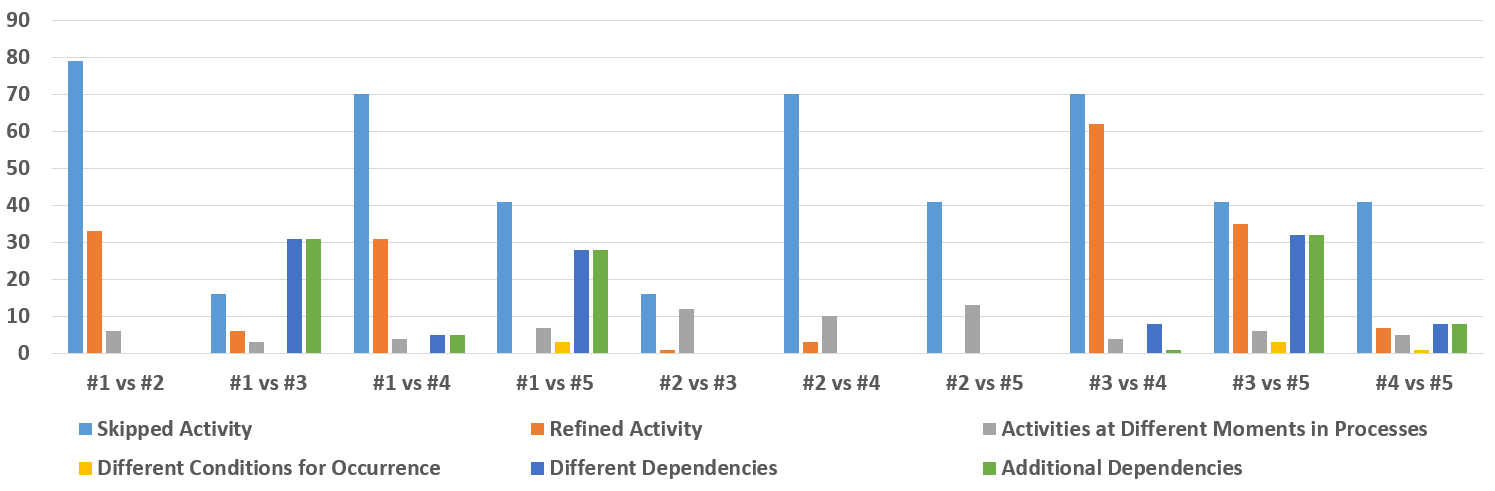
\includegraphics[width=\textwidth]{5_results_discussions/coselog-wabo/mismatch-pattern-types}
	\caption{Mismatch Pattern Types for Environmental Permit Application Process Dataset}
  \label{fig:coselog-wabo-mismatch-pattern-types}
\end{figure} 

In \textit{Recommendation Generation} stage, an organization and performance difference threshold is selected as analysis input likewise the previous dataset. For different threshold values, number of performance indicators that are performing better for the selected organization and spotted mismatch patterns are plotted in Figure~\ref{fig:coselog-wabo-recommendation-generation-analysis}. 
\begin{figure}
	\centering
	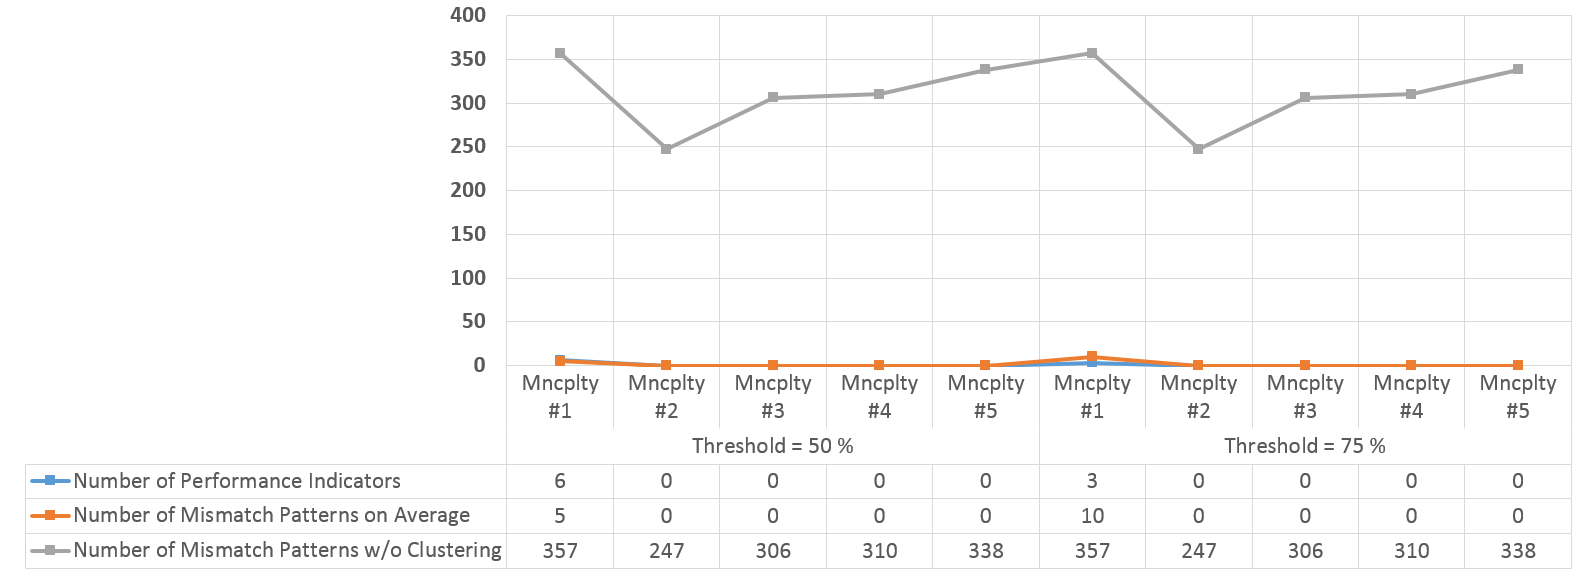
\includegraphics[width=\textwidth]{5_results_discussions/coselog-wabo/recommendation-generation-analysis}
	\caption{Recommendation Generation Analysis for Environmental Permit Application Process Dataset (2 Clusters)}
  \label{fig:coselog-wabo-recommendation-generation-analysis}
\end{figure}

In the analysis of Figure~\ref{fig:coselog-wabo-recommendation-generation-analysis}, it can be seen that only the cluster that the Municipality \#1 has the potential of learning from other cluster since it performs worse in performance indicators. For the threshold of 50\%, cluster of Municipality \#1 performs worse in 6 performance indicators and proposed approach lists total of 30 mismatch patterns. On the average it show 6 patterns to the user as the potential causes of performance improvement. With the same approach, cluster of Municipality \#1 performs worse in 3 indicators with the difference of 75 \% and on average 10 mismatch patterns are listed for each performance indicator. When it is compared to the total mismatch patterns of Municipality #1, which is 357, proposed approach helps significantly to the user for focusing performance improvement.

Since selecting number of clusters as 2 did not yield high learning potential for performance improvement, analysis is repeated with selecting number of clusters as 3. When three clusters are created, Municipality \#1 is located in the first cluster; Municipality \#2 and \#4 are located in the second cluster; and Municipality \#3 and \#5 are grouped in to the last cluster. For these clusters analysis is repeated for threshold of 25 \%, 50 \% and 75 \%, and as plotted in Figure~\ref{fig:coselog-wabo-recommendation-generation-analysis-k3}, in addition to Municipality \#1, now Municipality \#3 and \#5 have the learning potential from other clusters. However, Municipality \#2 and \#4 performs better in all performance indicators which yielded no mismatch pattern analysis data for them. Increasing cluster sizes in this analysis shows that organizations can learn more from each other but it has the potential danger of overfitting to other organizations process model. 
\begin{figure}
	\centering
	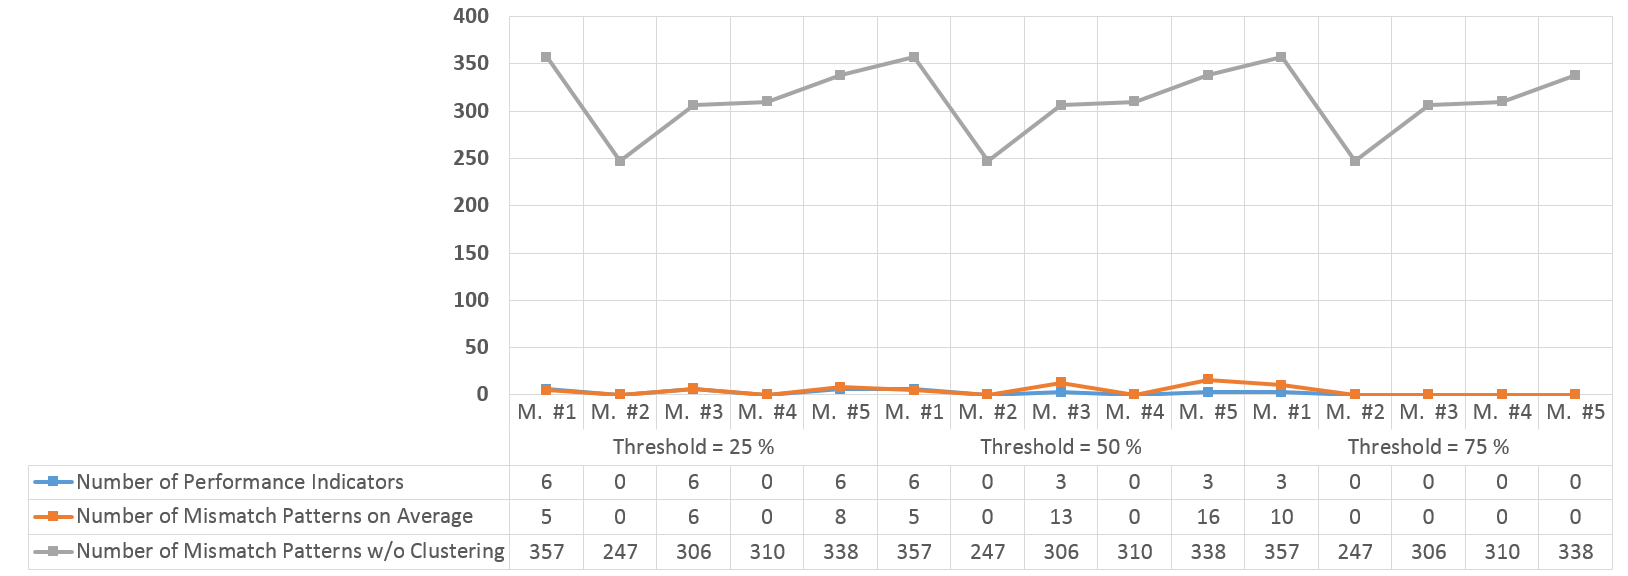
\includegraphics[width=\textwidth]{5_results_discussions/coselog-wabo/recommendation-generation-analysis-k3}
	\caption{Recommendation Generation Analysis for Environmental Permit Application Process Dataset (3 Clusters)}
  \label{fig:coselog-wabo-recommendation-generation-analysis-k3}
\end{figure}

\subsection{Discussions}
\label{sec:coselog-discussions}
\todo{write}
%evaluation metric'ler ve stage'lerin özetini geç
%çıkan sonuçların visual değerlendirmesini yap


\section{Discussions}
\label{sec:discussions}
When the evaluation of the stages for \textit{Loan Application Example} and \textit{Environmental Permit Application Process} datasets are gathered together, the following results can be expressed:

\begin{itemize}
	\item Process mining stage of the proposed methodology can mine the process models with perfect fitness and high appropriateness from event logs which have no noise. When the noise level increases in the dataset, fitness values of mined models decreases to 90 \% levels with a decreasing appropriateness of models.
	\item For the successfully mined models with high fitness values, replay and performance indicator calculation stage works seamlessly as expected. With this step, average and standard deviation time between each activity can be measured for each organization. Number of these metrics are quadratic to the number of activities in each organization's process model and difficult to analyze with a cross comparison.
	\item Internal measure of clusters indicates that the organizations can be clustered according to their performance indicators which emerges a collective understanding of organizations for their subprocesses. In other words, within-SSE values decrease significantly when the organizations are divided into clusters which shows that they can be grouped based on how well they are executing in their performance indicators.
	\item Mismatch analysis spots the differences between process models in coherence with structural similarity of them. This indicates that the idea of using mismatch patterns to reveal differences between process models is a feasible approach since its results are comparable to the similarity metrics of process models in the literature. However, only the total number of mismatch patterns are taken into consideration in this study where their importance and occurrence is variable. For instance, it can be a very useful information for a \textit{Skipped Activity} in a small dataset like \textit{Loan Application Example}; however it is very likely to see huge number of \textit{Skipped Activity} patterns in an immense dataset like \textit{Environmental Permit Application Process}. With this consideration, distributions of mismatch patterns are presented for each dataset to reveal any tendencies for occurrence. 
	\item Recommendation generation aims to gather all generated information in this thesis study to help focusing on the potentially important mismatch patterns for performance improvement. For this aim, different thresholds and different cluster sizes are analyzed to check responsiveness of this stage. When the number of mismatch patterns with and without performance clusterings are checked, it shows that in a small dataset, where even the mismatch patterns can be spotted by visual analysis, performance clustering lists 3 times less number of differences in \textit{Loan Application Example} dataset. When it is impossible to locate mismatch patterns manually like in \textit{Environmental Permit Application Process}, performance clustering spots 100 times less number of differences. This difference helps user to focus on the differences with a potential performance improvement which is one of the aims in this thesis study.
	\item Although each step of methodology can be counted as successful based on their evaluation metrics, mismatch patterns recommended at the end of methodology can yield important observations as well as being being irrelevant and infeasible. Since this decision is based on the business environment of organizations, quality of recommendations for business usefulness is out of the scope of this thesis study. However, some example recommendations can be presented to provide an insight:
	\begin{itemize}
	\item In the analysis of \textit{Loan Application Example}, for Variant \#3 performance clustering results indicate that other cluster of variants perform 27 \% better on average time and 12 \% better on standard deviation time between activities "Calculate Capacity" and "Accept". In other words, cluster of other variants complete the path between these activities in a short amount time with less variance. When the mismatch patterns for these performance indicators are checked the following ones can be mentioned:
		\begin{itemize}
		\item "Check Credit" is a \textit{Skipped Activity} in the other cluster.
		\item "Check Credit" is a \textit{Refined Activity} of with "Check System (50 \%)"; "Check Paper Archive (42 \%)"; "Send Credit Check Request (32 \%)"; "Process Credit Check Reply (31 \%)" where the corresponding similarity values provided in parentheses.
		\item "Calculate Capacity" is a \textit{Different Moments in Processes} which have different previous activities in clusters. 
		\end{itemize}
	When these example mismatch patterns are checked, removing "Check Credit" activity and putting other activities instead of it might be the cause of performance improvement. With the same approach, putting "Calculate Capacity" on different orders in processes can effect the average and variance of time to between activities. These mismatch patterns can also visualized on process model of Variant \#3 and a variant from other cluster in Figure~\ref{fig:loan-recommendation-visualization}. In the process models, refined activities of "Check Credit" and different positions of "Calculate Capacity" are indicated. 
		\begin{figure}
			\centering
			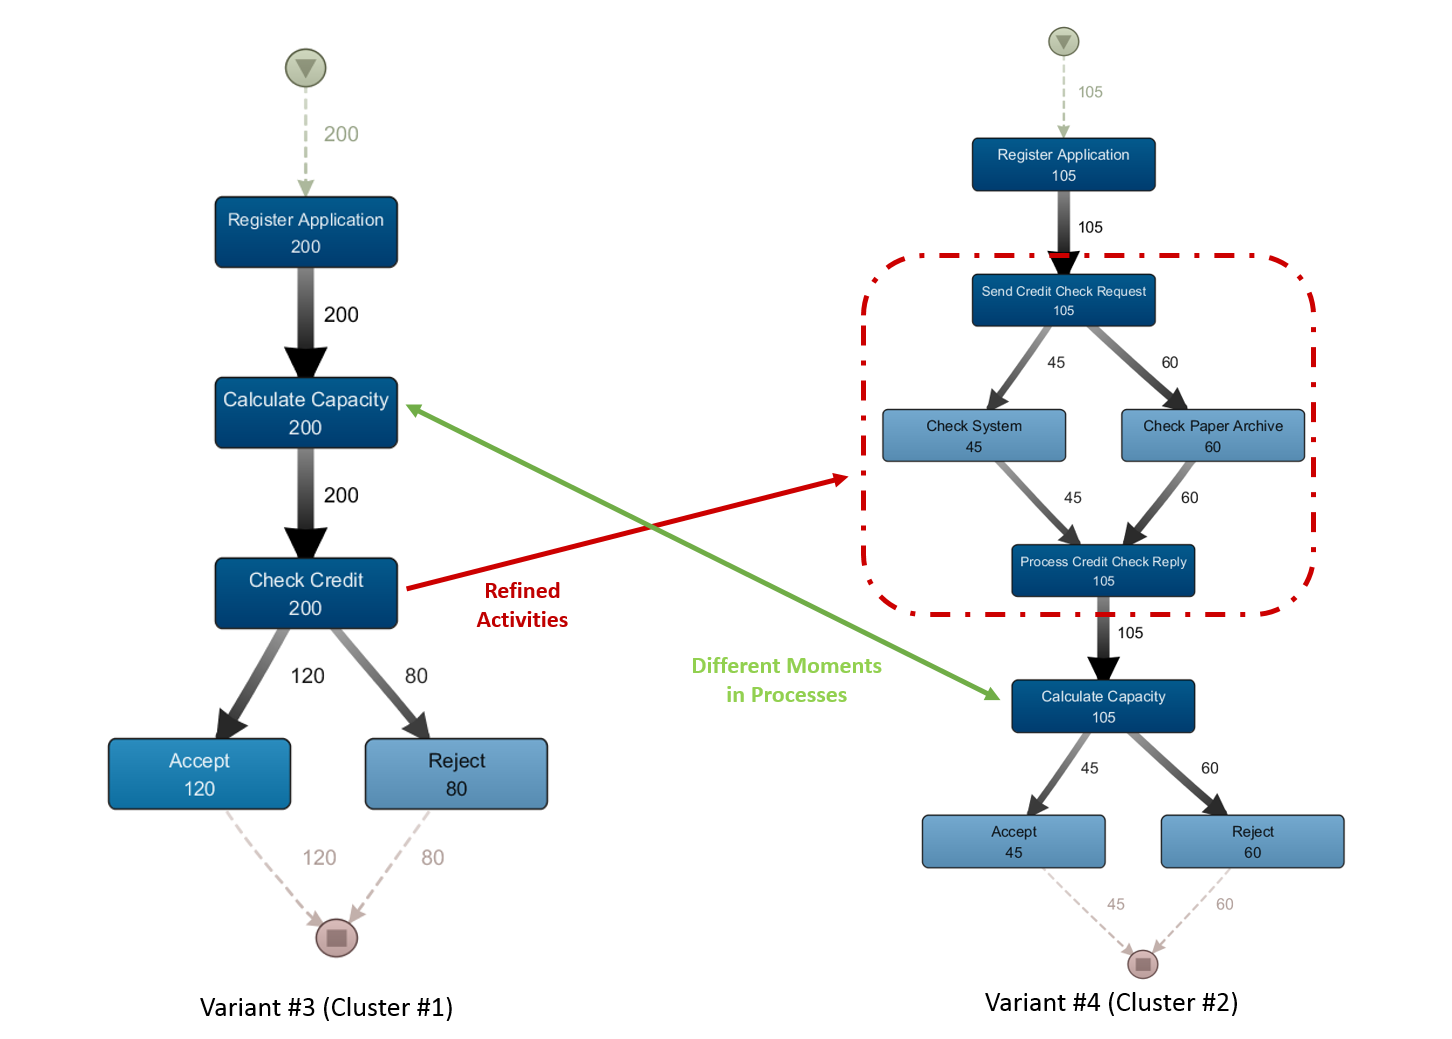
\includegraphics[width=\textwidth]{5_results_discussions/loan-application-process/recommendation-visualization}
			\caption{Visualization of example recommendation for Loan Application Process dataset}
		  \label{fig:loan-recommendation-visualization}
		\end{figure}
	\item In the analysis of \textit{Environmental Permit Application Process} with 3 clusters, Cluster \#3 performs 40 \% better on average time and 53 \% better on standard deviation time between the activities "01_HOOFD_010" and "01_HOOFD_015". When the mismatch patterns between these clusters for the performance indicator is listed the following ones can be mentioned:
		\begin{itemize}
			\item Activity "03_GBH_005" is a \textit{Different Moments in Processes} which have different next activities in clusters.
			\item Activity "01_HOOFD_015" is a \textit{Different Dependencies} and it has a different set of dependencies in clusters.
			\item Activity "16_LGSV_010" is a \textit{Different Moments in Processes} which have different next activities in clusters.
			\item Activity "01_HOODF_065" is a \textit{Different Dependencies} and it has a different set of precedence activities in different clusters.
 		\end{itemize}
	Although the activity codes in mismatch patterns do not reveal any information about their context, they are listed as potential cause of performance improvement. These mismatch patterns are also visualized on the fragments of process models in Figure~\ref{fig:coselog-wabo-recommendation-visualization-mun-5} and Figure~\ref{fig:coselog-wabo-recommendation-visualization-mun-5} since it is difficult to visualize the complete process models. In the process models, each mismatch pattern is marked and this shows how the proposed approach helps to focus on differences between process models.
			\begin{figure}
			\centering
			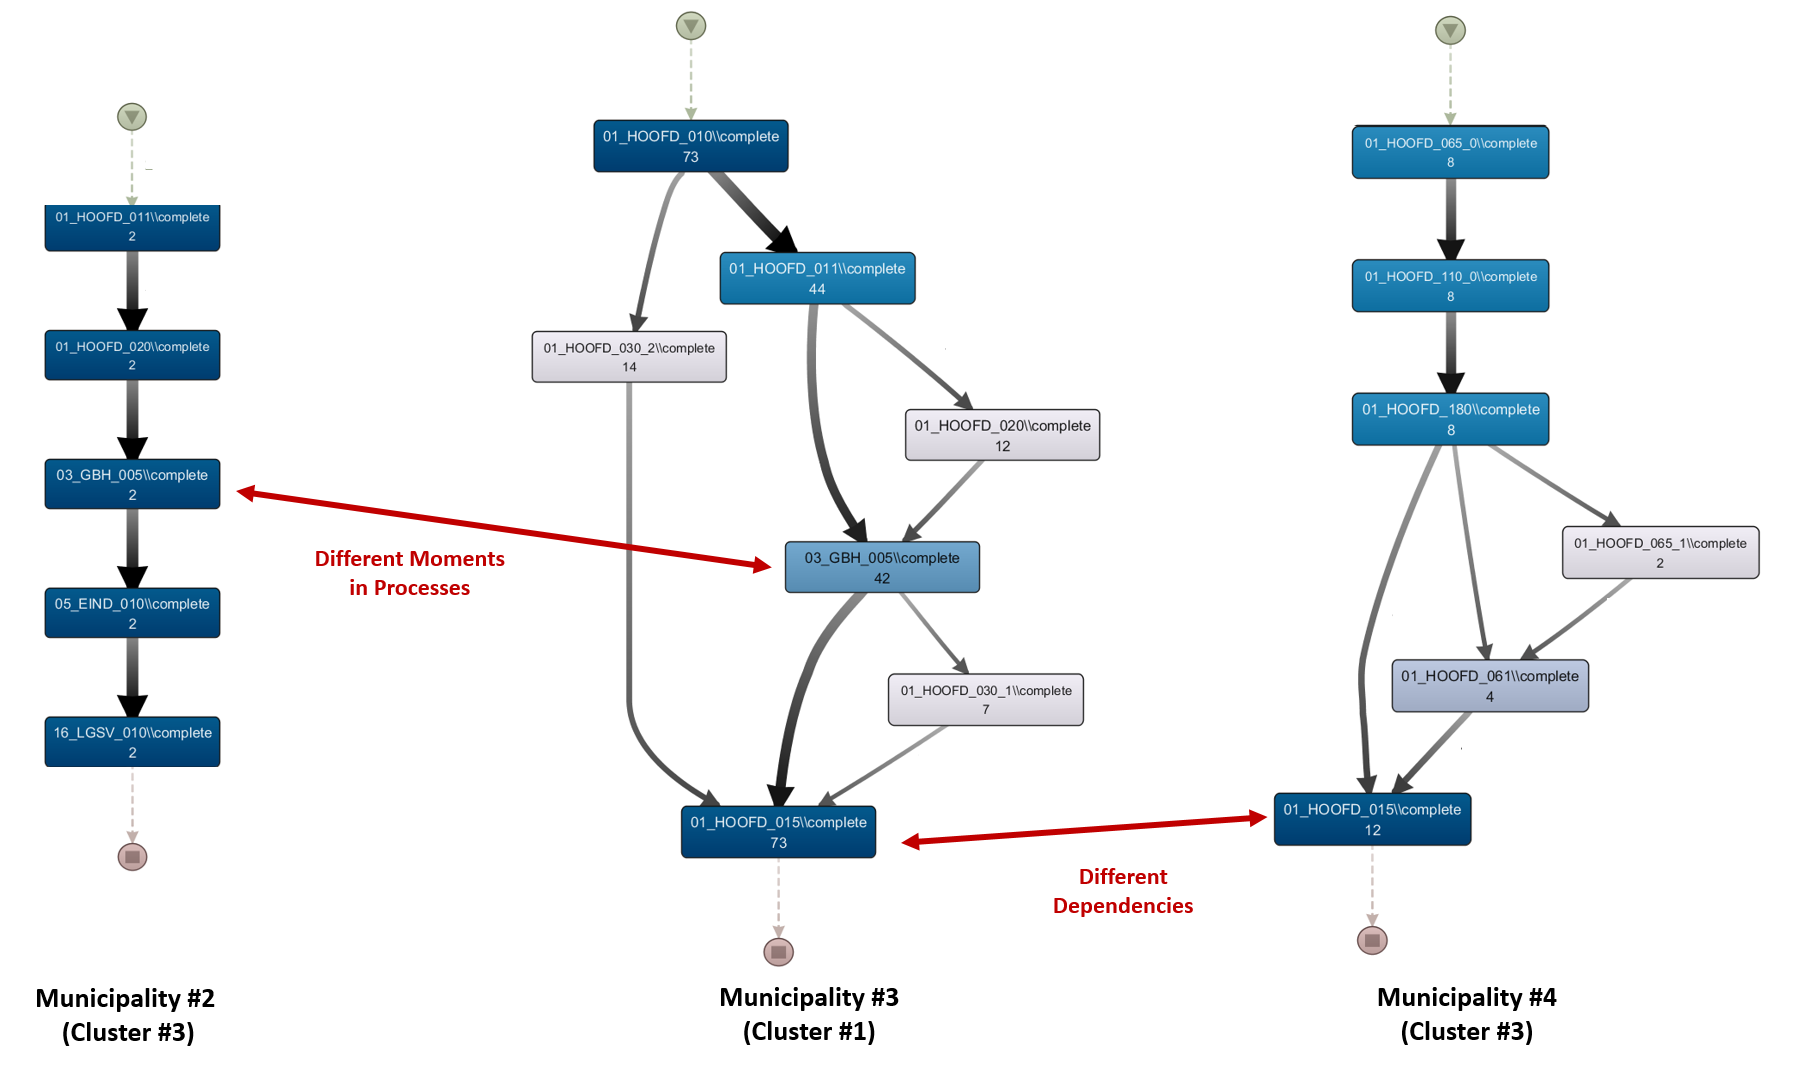
\includegraphics[width=\textwidth]{5_results_discussions/coselog-wabo/recommendation-visualization-mun-3}
			\caption{Visualization of example recommendation for Environmental Permit Application Process dataset (Municipality \#3)}
		  \label{fig:coselog-wabo-recommendation-visualization-mun-3}
		\end{figure}
				\begin{figure}
			\centering
			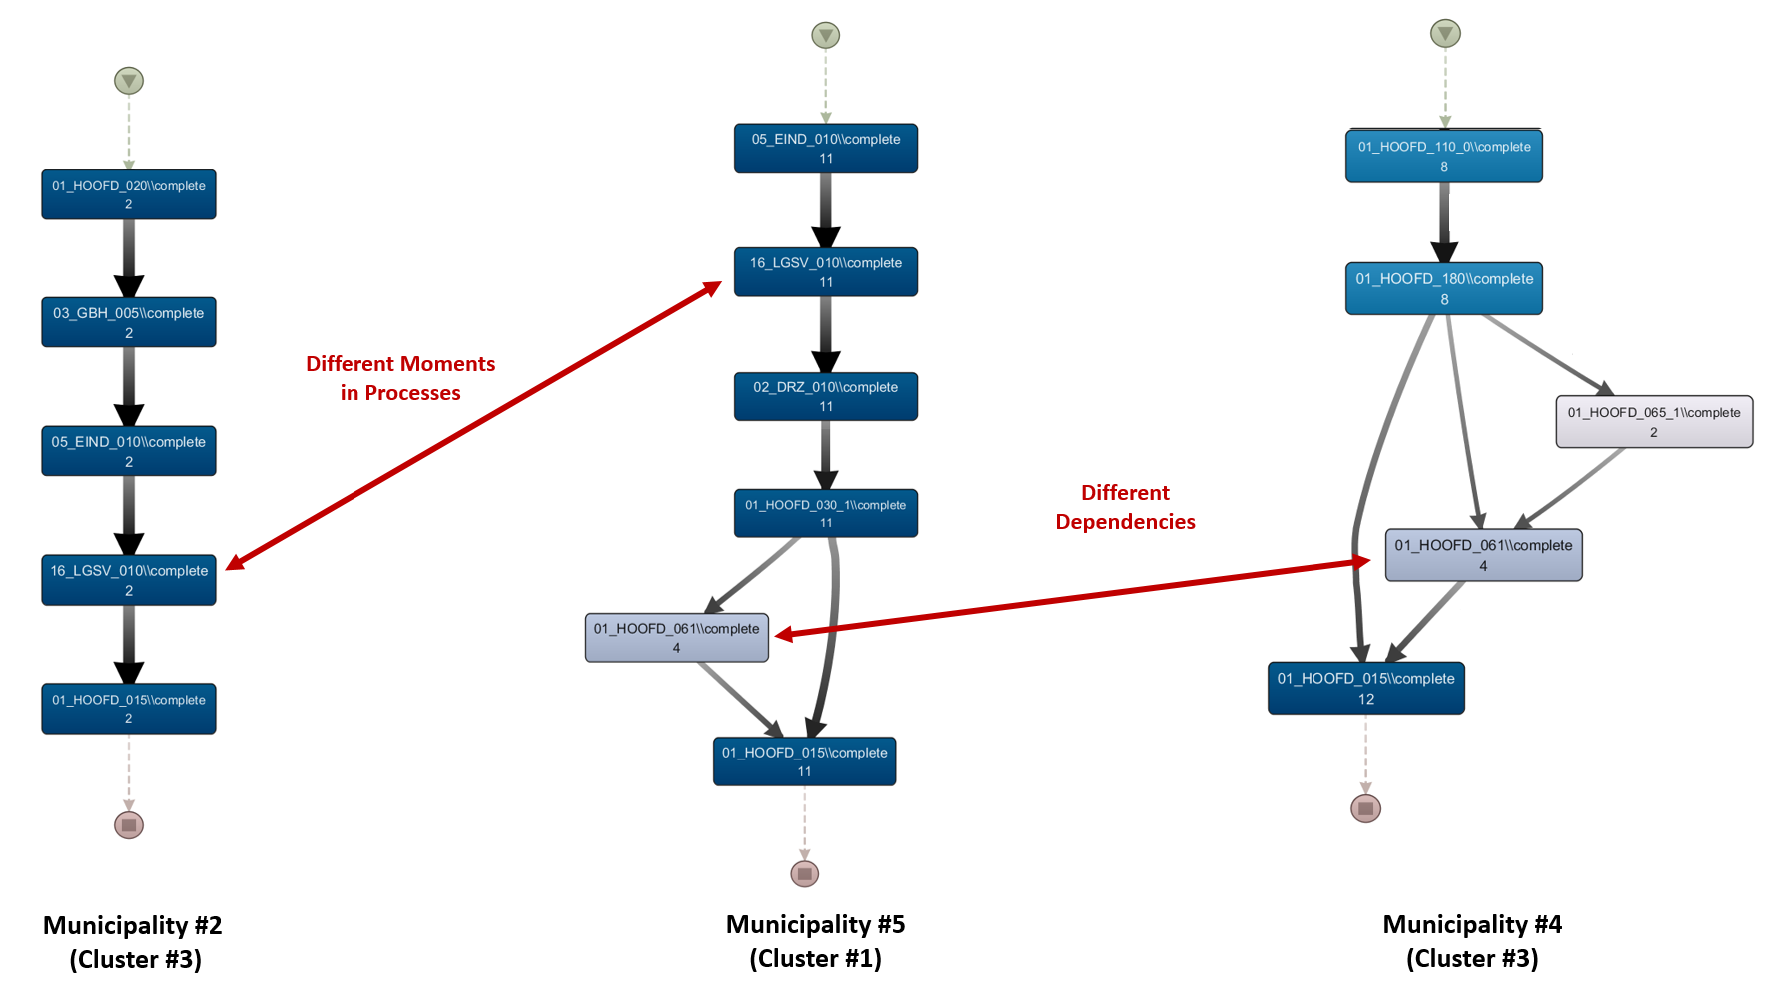
\includegraphics[width=\textwidth]{5_results_discussions/coselog-wabo/recommendation-visualization-mun-5}
			\caption{Visualization of example recommendation for Environmental Permit Application Process dataset (Municipality \#5)}
		  \label{fig:coselog-wabo-recommendation-visualization-mun-5}
		\end{figure}
	\end{itemize} % end of recommendations

\end{itemize} % end of discussions